% Este documento utiliza latex classes disponibilizadas
% no seguinte endereço: http://www.inf.ufrgs.br/utug

\documentclass[cic,tc]{iiufrgs}

\usepackage[brazilian]{babel}
\usepackage{graphicx}
\usepackage[T1]{fontenc}
\usepackage{times}
\usepackage{float}
\usepackage{setspace}
\usepackage{listings}
\usepackage{color}
\usepackage{tabularx}
\usepackage[utf8]{inputenc}
\usepackage[alf,abnt-emphasize=bf]{abntex2cite}	% pacote para usar citações abnt


\title{Rivers - Stream Processing API for Golang}

\author{Borges}{Diego}

\advisor[Prof.~Dr.]{Pimenta}{Marcelo}

\date{dezembro}{2015}

\course{Curso de Ciência da Computação}

\location{Porto Alegre}{RS}

\graphicspath{{images/}}
\DeclareGraphicsExtensions{.png,.pdf}

\renewcommand{\nominata}{
UNIVERSIDADE FEDERAL DO RIO GRANDE DO SUL
\par Reitor: Prof.~Dr.~Carlos Alexandre Netto
\par Vice-Reitor: Prof.~Dr.~Rui Vicente Oppermann
\par Pró-Reitor de Graduação: Prof.~Dr.~Sérgio Roberto Kieling
\par Diretor do Instituto de Informática: Prof.~Dr.~ Luís da Cunha Lamb
\par Coordenador do Curso de Ciência da Computação: Prof.~Dr.~Raul Fernando Weber
\par Bibliotecária-Chefe do Instituto de Informática: Beatriz Regina Bastos Haro
}

\keyword{API}
\keyword{rivers}
\keyword{golang}
\keyword{stream}
\keyword{pipeline}
\keyword{concurrency}

%
% ---------------------------------------------------------
%


\begin{document}

\maketitle

\clearpage
\begin{flushright}
\mbox{}\vfill
{\sffamily\itshape
``Do not communicate by sharing memory; instead, share memory by communicating''\\}
--- \textsc{Rob Pike}
\end{flushright}

\chapter*{Agradecimentos}
\label{cha:thanks}
TODO ...
TODO ...
TODO ...

%
% ---------------------------------------------------------
%

\tableofcontents

\begin{listofabbrv}{UFRGS}
    \item[API] Application Programming Interface
    \item[CPU] Central Processing Unit
    \item[FIFO] First In First Out
    \item[TCP] Transmission Control Protocol
    \item[UDP] User Datagram Protocol
    \item[HTTP] Hypertext Transfer Protocol
    \item[NoSQL] Non SQL
    \item[MVP] Minimum Viable Product
    \item[TDD] Test-Driven Development
    \item[HTML] HyperText Markup Language
    \item[URL] Uniform Resource Locator
\end{listofabbrv}

\listoffigures

\listoftables

\begin{abstract}
Nos últimos anos o poder computacional evoluiu drasticamente e os sistemas atuais podem beneficiar-se de CPUs com múltiplos cores para realizar concorrentemente tarefas de maneira mais eficiente.

Golang tira proveito do poder computacional de hardwares modernos implementando um modelo simple porém poderoso de concorrência baseado em troca de mensagens através de channels e um formato mais barato de thread gerenciado pelo runtime conhecido como goroutines.

Rivers propoem um framework para processamento de fluxo de dados utilizando o modelo de concorrência da linguagem Go como fundação e padrões bem conhecidos como Producer-Consumer e Go pipeline pattern provendo uma API fluente e extensível para criação e composição de pipelines complexos de processamento de dados aplicando conceitos de programação funcional.
\end{abstract}

\begin{englishabstract}{Rivers - Stream Processing API for Golang}{API, rivers, golang, stream, pipeline, concurrency}
During the past few years hardware power has evolved drastically and today's systems can leverage multi-core CPUs in order to perform concurrent tasks more effectively.

Golang takes advantage of this hardware power by implementing a simple though extremely powerful concurrency model built on top of concepts such as message passing via channels and a more lightweight form of thread managed by the runtime known as goroutines.

Rivers proposes a framework for data stream processing built on top of Go's concurrency model along with well known patterns such as the Producer-Consumer pattern and the Go pipeline pattern in order to provide a fluent and extensible API for building and composing complex data processing pipelines through functional programming concepts.
\end{englishabstract}

\onehalfspacing

\chapter{Introdução}
\label{cha:introduction}

\section{Motivação}
\label{sec:motivation}

Nos últimos anos a necessidade de se processar grandes volumes de dados de maneira eficiente e flexível tem aumentado drasticamente. Isso se deve ao fato de que sistemas computacionais estão cada vez mais complexos e frequentemente envolvem a colaboração entre diversos outros sistemas que atuam como fonte ou consumidores de dados. O fato de que as pessoas estão cada vez mais conectadas aos seus dispositivos móveis coletando e produzindo dados a todo momento é um dos indícios dessa crescente complexidade que tende a continuar à medida que novas tecnologias são introduzidas como por exemplo Iternet of Things \cite{blog:iot:council}, aumentando ainda mais a quantidade de dados produzidos e com isso a necessidade de se processar e comunicar estes dados entre os diferentes sistemas que compõem o que conhecemos como Internet.

Dados são gerados assincronamente por diversas fontes como por exemplo aplicativos móveis, sensores, sistemas web e fluem de um sistema à outro através de mecanismos de comunicação tais como APIs e Push Notifications \cite{docs:apple:push_notification} passando por transformações, filtros e agregações para se adequar ao contexto e as necessidades de cada sistema. Todo este processamento quando aplicado a grandes quantidades de dados em um contexto de sistemas distribuídos torna-se surpreendentemente desafiador. Várias soluções foram propostas nos últimos anos para abordar o processamento assíncrono de grandes volume de dados dentre elas o processamento de streams, solução explorada por este trabalho no contexto da linguagem de programação Go da google.

A decisão pelo uso da linguagem de programação Go se deve à alguns fatores. Go introduz um modelo de concorrência poderoso e simples baseado em troca de mensagens através da colaboração entre channels \ref{subsec:channels} e goroutines \ref{subsec:goroutines} permitindo um único programa executar centenas de milhares de fluxos concorrentes de execução com o mínimo de overhead, o que a torna uma linguagem extremamente atraente no contexto de processamento de streams. Go tem ganhado notável adoção na comunidade de desenvolvedores tanto pela simplicidade da linguagem que permite com que soluções elegantes sejam empregadas à problemas complexos como no desenvolvimento de web servers, aplicações que fazem intenso uso de mecanismos de comunicação de rede como TCP e UDP, parsers e etc. No entanto, a linguagem não provê abstrações nativas para o processamento de streams tornando o trabalhado de um desenvolvedor não necessariamente trivial.

\section{Objetivos}
\label{sec:objectives}

Este trabalho tem como principal objetivo a implementação de uma API  simples e flexível para processamento de streams através da abstração de pipelines para a linguagem de programação Go da google. A solução proposta tem como base teórica conceitos do modelo Produtor-Consumidor \cite{paper:david_kocher:producer_consumer} juntamente com conceitos de programação funcional tais como Collection Pipeline definido em \cite{article:martin_fowler:collection_pipeline}. Em sua fundação prática, a solução explora o modelo de concorrência da linguagem Go afim de usufruir ao máximo dos recursos de hardware visando atingir níveis extremos de concorrência e paralelismo.

Visando o reuso de código, a API proposta disponibiliza um conjunto mínimo de abstrações para cada um dos conceitos envolvidos na criação de um pipeline e seus estágios de processamento de stream que servirão como base para a implementação de componentes mais complexos e especializados, tais como mecanismos básicos para a produção de dados de diversas fontes como por exemplo arquivos, sockets e listas e também componentes especializados em operações de transformações de dados como por exemplo Map, Reduce, Filter encontradas em outras soluções similares discutidas no capítulo \ref{cha:related_work}. Afim de adequar-se a cenários não inicialmente previstos Rivers disponibiliza mecanismos para que abstrações nativas da API possam ser estendidas com novas implementações permitindo a criação de pipelines para o processamento de qualquer tipo de dados independente de sua origem.

Finalmente a API proposta seguindo conceitos de programação funcional deve permitir que estágios do pipeline possam ser combinados de maneira simples tal que dados produzidos por um estágio possam ser consumidos por um próximo estágio de maneira assíncrona e concorrente, sendo possível porém opcional a paralelização de estágios específicos afim de aumentar a eficiência de processamento de dados de um estágio em particular.

\begin{flushright}
\mbox{}\vfill
{\sffamily\itshape
``Any fool can write code that a computer can understand. Good programmers write code that humans can understand.''\\}
--- \textsc{Martin Fowler, 2008}
\end{flushright}

\section{Estrutura do Texto}
\label{sec:text_structure}

Este trabalho está organizado em sete capítulos os quais abordam temas relevantes para o entendimento das decisões tomadas no processo de desenvolvimento da solução e suas motivações assim como definição de conceitos básicos utilizados como fundação do trabalho. A seguir cada capítulo é apresentado de maneira mais detalhada.

\begin{description}
    \item [Capítulo~\ref{cha:introduction}] Apresenta o contexto em que o trabalho foi desenvolvido as motivações que justificam a solução proposta assim como seus objetivos.
    \item [Capítulo~\ref{cha:foundation}] Descreve os termos e conceitos básicos utilizados como fundação do trabalho dando suporte teórico e prático para a solução proposta.
    \item [Capítulo~\ref{cha:related_work}] Discute alguns trabalhos relacionados que serviram de base e inspiração para muitas das decisões técnicas tomadas ao longo do processo de desenvolvimento deste trabalho.
    \item [Capítulo~\ref{cha:rivers}] Apresenta a solução proposta em detalhes assim como a arquitetura desenvolvida e seus componentes internos
    \item [Capítulo~\ref{cha:rivers_implementation}] Descreve o processo de desenvolvimento empregado assim como as práticas utilizadas para a validação gradual de requisitos assim como a integração contínua e constante da implementação empregada.
    \item [Capítulo~\ref{cha:applications}] Apresenta alguns casos de uso detectados ao longo do desenvolvimento assim como aplicações reais da solução em ambientes de produção juntamente como a visão de desenvolvedores que fizeram para da validação deste trabalho.
    \item [Capítulo~\ref{cha:conclusion}] Por fim, são apresentados as conclusões, resultados e algumas considerações finais com relação a possíveis melhorias e avanços futuros.
\end{description}

\chapter{Fundamentos}
\label{cha:foundation}

Neste capítulo serão discutidos alguns conceitos básicos utilizados como fundação no desenvolvimento da solução assim como alguns detalhes técnicos relacionados a linguagem de programação Go necessários para o entendimento dos mecanismos implementados em Rivers e discutidos em capítulos seguintes.

\section{Streams}
\label{sec:streams}

Streams são definidos como uma sequência de dados que são produzidos assincronamente ao longo do tempo fluindo de sua fonte conhecida como upstream à um destino chamado de downstream \cite{article:tim:streams}. Frequentemente streams são comparados à coleções de dados como por exemplo arrays e listas. No entanto streams diferentemente de coleções não definem necessariamente um tamanho fixo, podendo produzir elementos indefinidamente ao longo do ciclo de vida de um programa. Apesar desta diferença, as APIs de streams são muitas vezes modeladas de maneira que se assemelham a APIs de manipulação de coleções compartilhando muitas das operações como \emph{filter}, \emph{map}, \emph{reduce} etc.

Streams são amplamente aplicados no âmbito computacional no entanto em muitos casos seus conceitos não são explicitamente aparentes. Um exemplo clássico são os \emph{Unix Pipes}, mecanismos utilizados para realizar comunicação entre processos \cite{book:tanenbaum:ipc} via canais de comunicação conhecidos como standard input e output ou simplesmente \emph{stdin} e \emph{stdout} respectivamente. Uma operação de pipe conecta o canal stdout de um programa ao stdin de outro permitindo com que dados sejam transmitidos de um lado ao outro passando por diferentes estágios de processamento específicos a cada programa. A figura \ref{fig:unix_pipes} mostra os comandos Unix \emph{find}, \emph{grep} e \emph{wc} sendo combinados via operações de \emph{pipe} formando um pipeline com três estágios de processamento.

As aplicações de streams são tantas que muitas linguagens de programação adotam completamente os seus conceitos e disponibilizam APIs robustas que permitem a criação de pipelines complexos de processamento de stream de dados, alguns exemplos são \cite{docs:nodejs:streams}, \cite{docs:haskell:streams} e \cite{docs:java8:streams}.

\begin{figure}[H]
  \includegraphics[width=0.55\textwidth]{unix-pipes}
  \centering
  \caption{Exemplo de stream pipeline em Unix.}
  \label{fig:unix_pipes}
\end{figure}

\section{Golang}
\label{sec:golang}

Go é uma linguagem de programação open source, estaticamente tipada \cite{paper:microsoft:static_typing} com suporte a garbage collector \cite{paper:sun:gc} criada pela Google com foco em simplicidade, produtividade e concorrência. O sistema de tipos da linguagem aborda de maneira inovadora alguns conceitos como por exemplo interfaces \cite{article:wikipedia:interfaces} que difere do conceito tradicional implementado por linguagens como Java. Outro aspecto interessante da linguagem é seu modelo de concorrência baseado em Goroutines \cite{docs:golang:goroutine} conceito similar ao de Coroutines \cite{article:wikipedia:coroutines} e troca de mensagens \cite{lecture:ucl:message_passing} através do uso de canais de comunicação. A seguir serão apresentados alguns dos conceitos da linguagem que foram essenciais na implementação de Rivers.

\subsection{Interfaces}
\label{subsec:interfaces}

Interface é o mecanismo através do qual sistemas podem ser modelados visando reuso e extensibilidade. Contratos abstratos são especificados descrevendo determinadas funcionalidades de um sistema independente de possíveis implementações, isso permite com que qualquer componente satisfazendo uma determinada interface possa ser utilizado como provedor da funcionalidade em questão. Em muitas linguagens de programação como Java, componentes precisam explicitamente declarar sua intenção de implementar uma interface e com isso sendo necessário definir as interfaces necessárias de um sistema como parte da modelagem da solução e consequentemente tornando a solução menos suscetível a futuras alterações de design. O código \ref{code:java:interfaces} mostra um exemplo de uma classe Java implementando uma interface específica.

\begin{figure}[H]
  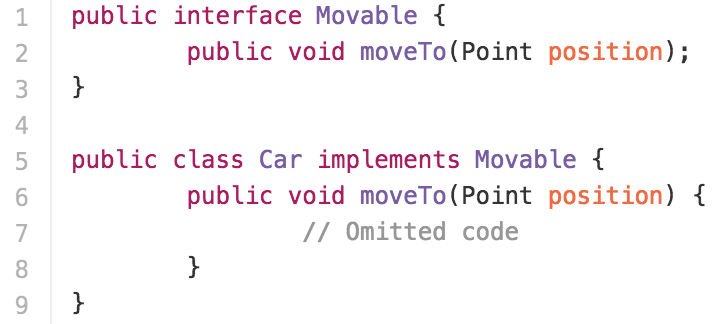
\includegraphics[width=0.65\textwidth]{java_interfaces}
  \centering
  \caption{Exemplo de implementação de uma interface em Java.}
  \label{code:java:interfaces}
\end{figure}

Em Go, interfaces são satisfeitas implicitamente sem a necessidade de que componentes declararem explicitamente sua intenção de implementar uma interface eliminando assim hierarquias de dependências presentes em linguagens orientadas à objetos \cite{book:learn_oop}. Para que um componente A satisfaça a interface B, A deve simplesmente implementar todos os métodos declarados em B. Desta maneira decisões arquiteturais de sistema podem ser tomadas em momentos futuros a medida em que novos casos de uso são introduzidos e padrões de código detectados evoluindo assim a arquitetura gradativamente. O código a seguir mostra como o exemplo Java em \ref{code:java:interfaces} pode ser reescrito em Go. Note que o tipo Car não possui qualquer dependência com a interface Movable ao contrário da versão Java, porém pode ser utilizado como um tipo Movable por implementar o método MoveTo na linha 7.

\begin{figure}[H]
  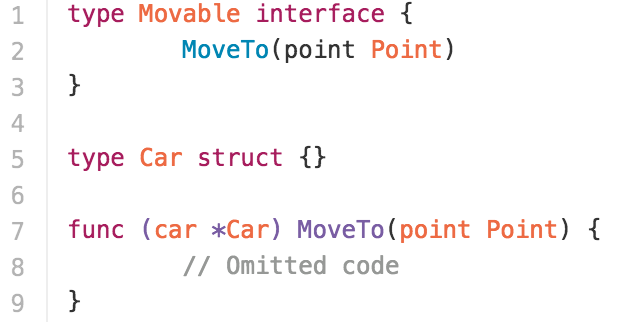
\includegraphics[width=0.5\textwidth]{go_interfaces}
  \centering
  \caption{Exemplo de implementação de uma interface em Go.}
  \label{code:go:interfaces}
\end{figure}

Em \ref{sec:rivers:architecture} será discutido como Rivers faz o uso de interfaces para definir os building blocks do framework permitindo novas funcionalidades sejam introduzidas à arquitetura de maneira transparente e não intrusiva.

\begin{flushright}
\mbox{}\vfill
{\sffamily\itshape
``Note too that the elimination of the type hierarchy also eliminates a form of dependency hierarchy. Interface satisfaction allows the program to grow organically without predetermined contracts. And it is a linear form of growth; a change to an interface affects only the immediate clients of that interface; there is no subtree to update. The lack of implements declarations disturbs some people but it enables programs to grow naturally, gracefully, and safely.
''\\}
--- \textsc{Rob Pike}
\end{flushright}

\subsection{Goroutines}
\label{subsec:goroutines}

Goroutine é o mecanismo que a linguagem Go utiliza para executar código de maneira concorrente e potencialmente em paralelo de maneira similar a outros mecanismos como por exemplo \cite{article:wikipedia:coroutines} e \cite{article:wikipedia:threads} porém com algumas diferenças que faz com que seu papel no modelo de concorrência da linguagem seja crucial. Goroutines são basicamente funções que executam assincronamente e concorrentemente utilizando o comando go e são gerenciadas pelo runtime da linguagem. Ao contrário de threads que exigem pelo menos 1MB de memória inicial para inicialização, Goroutines são extremamente baratas sendo necessário apenas 2KB de memória para inicialização podendo ajustar este valor sob demanda alocando e desalocando espaço na Heap, permitindo com que centenas de milhares de Goroutines possam ser executadas concorrentemente. Além disso o custo de troca de contexto entre Goroutines é extremamente baixo comparado com threads uma vez que Goroutines são genrenciadas pelo runtime e ao contrário de threads não necessitam acessar recursos do Sistema Operacional para realizar a troca de contexto. \cite{blog:how_goroutines_work} faz uma excelente análise do funcionamento de Goroutines em comparação com o funcionamento de OS threads. A figura \ref{code:goroutine:example} mostra uma Goroutine sendo criada na linha 16 utilizando o comando go para executar assincronamente a função say com o parâmetro "world".

\begin{figure}[H]
  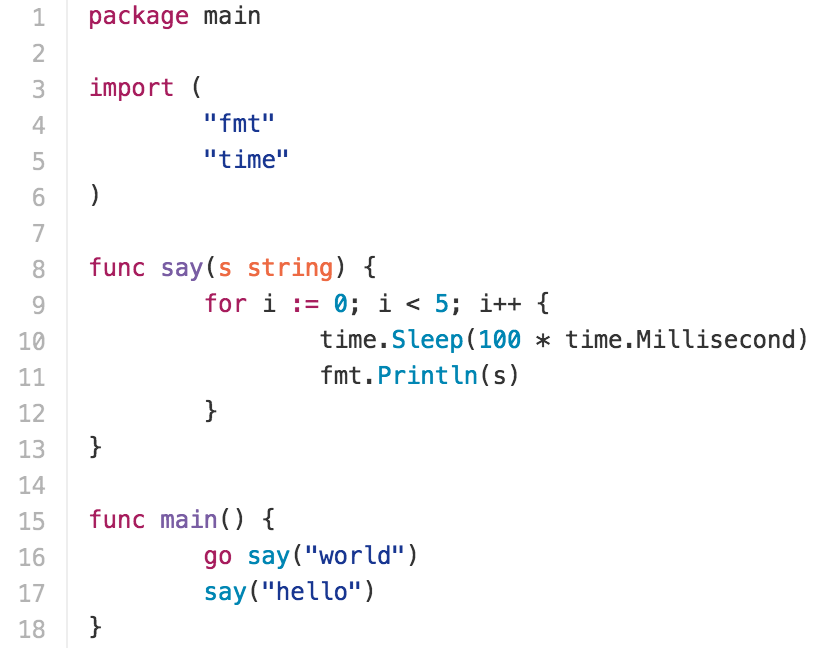
\includegraphics[width=0.75\textwidth]{goroutine_example}
  \centering
  \caption{Exemplo de uso de Goroutines.}
  \label{code:goroutine:example}
\end{figure}

\subsection{Channels}
\label{subsec:channels}

Channel é o mecanismo básico utilizado para realizar a comunicação entre Goroutines via troca de mensagem e a sincronização de suas execuções permitindo que dados sejam enviados de uma Goroutine à outra de maneira segura sem a necessidade de compartilhar memória e é a base para o modelo Produtor-Consumidor \cite{paper:david_kocher:producer_consumer} utilizado como fundação na implementação de Rivers.

Dados são escritos e lidos de um Channel de maneira síncrona sendo desnecessário o uso de outras primitivas de concorrência como por exemplo semáforos ou mutex \cite{paper:concurrency:schmidt}. Por padrão uma Goroutine ao escrever um dado em um Channel bloqueia sua execução até que outra Goroutine leia este dado do Channel liberando espaço para que outro dado seja escrito. No entanto um Channel pode ser criado com um Buffer permitindo com que vários dados possam ser escritos no Channel sem que sejam consumidos, bloqueando então apenas quando não houver mais espaço no Buffer. Channels podem ser de somente escrita, somente leitura ou ambos permitindo implementar alguns padrões de design interessantes como por exemplo Pipeline Pattern \cite{docs:golang:pipeline_pattern}. A figura a seguir mostra um exemplo de criação de um Channel com um Buffer de capacidade 2 na linha 2 e duas mensagens enviadas no canal nas linhas 3 e 4 e logo em seguida consumidas nas linhas 6 e 7. 

\begin{figure}[H]
  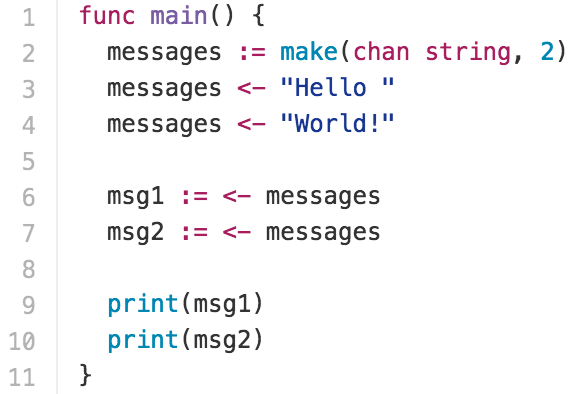
\includegraphics[width=0.55\textwidth]{channels_example}
  \centering
  \caption{Exemplo de uso de Channels.}
  \label{code:channels:example}
\end{figure}


\chapter{Trabalhos Relacionados}
\label{cha:related_work}

A seguir serão descritos brevemente alguns projetos que inspiraram a criação de Rivers não necessariamente relacionados à linguagem Go mas que aplicam conceitos similares para processamento de dados frequentemente no formato de streams.

\section{Apache Spark}
\label{sec:apache_spark}

Achache Spark \cite{docs:apache:spark} é uma solução para computação de tempo real, tolerante a falhas e com suporte a clustering \cite{article:kris:clustering}, com APIs em diferentes linguagens de programação como por exemplo scala, java e python. Spark tornou-se muito popular em áreas de \emph{Machine Learning} \cite{course:coursera:ml} e \emph{Analytics} \cite{article:techtarget:analytics} devido ao seu grande poder computacional que permite que grandes volumes de dados possam ser processados e distribuídos em diferentes máquinas de um cluster sendo uma solução muito atrativa também para sistemas de processamento de eventos \cite{docs:apache:streaming}.

\begin{figure}[H]
  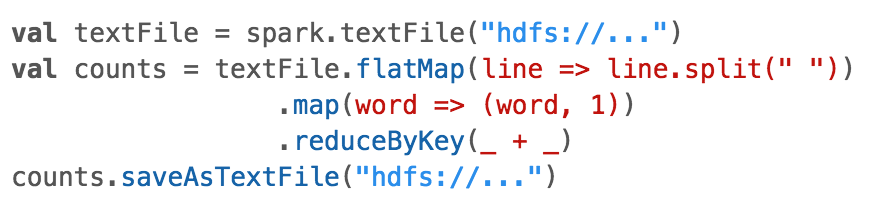
\includegraphics[width=0.7\textwidth]{spark}
  \centering
  \caption{Exemplo de uso da API scala de Spark.}
  \label{code:apache:spark}
\end{figure}

A API de Rivers é fortemente inspirada na fluência da API Spark, aplicando \emph{Method Chaining} \cite{article:sitepoint:method_chaining} sempre que possível aumentando a legibilidade do código resultante. Ambas APIs aplicam ao máximo os conceitos de programação funcional disponibilizando operações de filtros, mapeadores e agregadores de dados provendo um considerável nível de composição entre operações permitindo a criação de pipelines complexos de processamento de streams fortemente suscetíveis ao reuso. Suporte à clustering em Rivers é proposto como parte de trabalhos futuros.

\section{Java 8 Streams}
\label{sec:java8_streams}

A versão 8 da linguagem de programação Java introduz a abstração de Streams \cite{docs:java8:streams} como parte de suas bibliotecas padrão e assim como outras linguagens e plataformas como Spark, disponibiliza uma API fluente baseada em conceitos de programação funcional, permitindo a criação de pipelines para processamento de streams com suporte a paralelização. Assim como Spark, a API de streams de Java8 contribuíram para o design da API de Rivers afim de prover uma API similar para a linguagem Go que não fosse somente simples porém familiar à desenvolvedores com conhecimentos de programação funcional e extensível permitindo que a solução fosse aplicada à novos casos de uso introduzindo implementações diferentes dos componentes básicos do framework \ref{sec:rivers:building_blocks}.

\begin{figure}[H]
  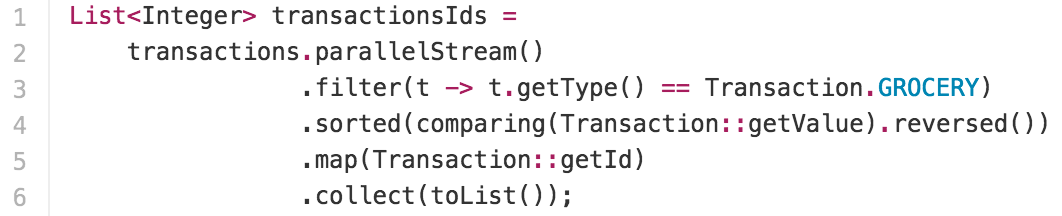
\includegraphics[width=0.9\textwidth]{java8_streams}
  \centering
  \caption{Exemplo de uso da API de streams em Java8.}
  \label{code:java8:streams}
\end{figure}

\section{ReactiveX - Reactive eXtensions}
\label{sec:reactive_extensions}

\emph{Reactive eXtensions} \cite{docs:reactivex:streams} é um movimento que tomou tração nos últimos anos liderado por empresas como \cite{netflix} e \cite{microsoft} dentre outras que procura tornar \emph{mainstream} conceitos de programação reativa \cite{article:reactive_programming} empregando vários conceitos de programação funcional e conhecidos padrões de design como \emph{Observer Pattern} \cite{article:pattern:observer} e \emph{Observable Pattern} \cite{article:pattern:observable} na criação de APIs assíncronas para tratamento de fluxo de dados. Estes conceitos quando combinados permitem com que APIs poderosas sejam implementadas abstraindo muito dos desafios envolvidos na programação assíncrona como por exemplo sincronização de threads, estruturas de dados concorrentes e operações de IO não bloqueantes. Existem várias implementações da especificação dentre elas estão a API Java \cite{docs:javarx} e Javascript \cite{docs:javascriptrx}.

Apesar de Rivers não seguir necessariamente a especificação de Reactive eXtensions, muitas decisões de design em Rivers foram baseados em conceitos similares aplicados à RX, como por exemplo realização de \emph{back-pressure} \cite{article:tim:streams} do pipeline através da utilização de Go \emph{buffered channels} \cite{docs:go:buffered_channels}. Reactive eXtensions e outros casos de uso explorados neste capítulo mostram que processamento de streams é uma solução interessante para muitos problemas relacionados a diversas áreas tecnológicas como por exemplo Big Data, Analytics, Event Processing e muitas linguagens de programação adotaram estes conceitos de provendo APIs nativas que permitem com que pipeline de processamento de streams sejam criados de maneira simples abstraindo muito dos desafios envolvidos com relação a concorrência e paralelização de um pipeline por exemplo, motivando a criação de Rivers.

\begin{flushright}
\mbox{}\vfill
{\sffamily\itshape
``ReactiveX is more than an API, it's an idea and a breakthrough in programming. It has inspired several other APIs, frameworks, and even programming languages.''\\}
--- \textsc{ReactiveX.io}
\end{flushright}


\chapter{Rivers}
\label{cha:rivers}

\section{Arquitetura}
\label{sec:rivers:architecture}

A arquitetura Rivers foi modelada com o intuito de prover uma API simples, flexível e extensível para a criação de pipelines complexos de processamento de stream de dados, tendo como fundação princípios do modelo produtor-consumidor aplicados ao modelo de concorrência da linguagem Go juntamente com o design pattern Pipeline e conceitos de programação funcional. Rivers faz uso de goroutines para o processamento concorrente e assíncrono de cada estágio do pipeline e channels para realizar a comunicação entre os mesmos. Afim de promover reuso e extensibilidade a API é definida em termos de Go interfaces disponibilizadas no pacote stream juntamente com componentes pré-definidos que podem ser combinados para criação de pipelines desde os mais simples até os mais complexos com mecanismos de fork e join por exemplo.

Rivers pipelines frequentemente são compostos por um estágio inicial conhecido como Producer \ref{sec:rivers:producers} responsável por gerar assincronamente os dados a serem processados. Opcionalmente, um pipeline pode ter um ou mais estágios intermediários conhecidos como Transformers \ref{sec:rivers:transformers} responsáveis por transformar os dados que passam por eles aplicando funções tais como filtros e flatmaps disponibilizando o resultado em um stream de leitura para que o próximo estágio possa consumi-lo de maneira assíncrona. O último estágio de um pipeline é representado por um Consumer \ref{sec:rivers:consumers} que bloqueia a execução do programa até que todos os dados sejam consumidos e o pipeline encerrado. Este último estágio ao fim da execução coleta e retorna qualquer eventual erro durante a execução para que o mesmo possa ser tratá-lo apropriadamente. Cada estágio do pipeline é conectado sequencialmente a um estágio seguinte utilizando streams de escrita e leitura conhecidos respectivamente por Writable e Readable \ref{sec:rivers:streams}. Estágios produzindo dados como producers e transformers escrevem estes valores em um stream de escrita, disponibilizando a versão de leitura deste stream à um próximo estágio para que este possa consumi-lo de maneira assíncrona.

Estágios do pipeline compartilham um mesmo contexto de execução utilizado para coordenar o fluxo de dados e sinalizar o término prematuro do pipeline devido a uma operação de short-circuit \cite{article:wikipedia:short_circuit_evaluation} ou devido a falhas ocorridas em algum ponto da execução. Este mecanismo permite com que cada estágio verifique o estado atual do pipeline antes de iniciar qualquer processamento podendo finalizar sua execução caso o pipeline tenha sido encerrado. Em situações aonde o contexto de execução é finalizado devido a erros, cada estágio do pipeline deve garantir que qualquer recurso sendo utilizado seja liberado corretamente como descritores de arquivos, channels, conexões com base de dados, etc. Um estágio pode requisitar o término do contexto de execução devido a uma falha ou pelo término prematuro como mencionado nos casos de operações de short-circuit. Este mecanismo permite que dowstreams do pipeline possam notificar upstreams com relação ao término da execução finalizando a produção de dados.

O diagrama \ref{fig:rivers:pipeline} mostra a relação entre estes componentes de um pipeline e sua representação equivalente em código Go.

\begin{figure}[H]
  \includegraphics[width=0.7\textwidth]{pipeline}
  \centering
  \caption{Rivers Pipeline.}
  \label{fig:rivers:pipeline}
\end{figure}

Pipelines podem assumir estruturas bem complexas como mencionado anteriormente. Rivers provê mecanismos para combinar múltiplos streams assim como duplicar um stream em vários outros. Estes mecanismos são conhecidos como Combiners e Dispatchers respectivamente e permitem a construção de pipelines mais complexos com vários fluxos concorrentes de processamento. Combiners são muito convenientes em situações aonde dados são produzidos por fontes de dados diferentes porém devem ser processados por uma mesma sequência de operações. O diagrama \ref{fig:rivers:combiner} representa dois pipelines sendo combinados em um único através de uma operação de merge e seu resultado sendo processado por um Transformer e em seguida consumido por um Consumer.

\begin{figure}[H]
  \includegraphics[width=0.95\textwidth]{combiner}
  \centering
  \caption{Exemplo de Uso de Combiner.}
  \label{fig:rivers:combiner}
\end{figure}

Um Dispatcher por sua vez é útil para condicionalmente classificar e separar dados de um stream os quais podem ser processados separadamente por uma sequência de estágios do pipeline. Rivers fornece algumas implementações de Dispatchers como por exemplo as operações Partition e Split. A primeira particiona o stream em dois outros baseado em um predicado que é aplicado a cada elemento do stream retornando dois novos streams. Elementos que atendem o predicados são redirecionados ao primeiro stream e o restante redirecionados ao segundo stream. A operação de Split simplesmente duplica o stream em dois outros streams idênticos permitindo que diferentes sequências de operações possam ser aplicadas a um mesmo elemento. O diagrama a seguir representa um pipeline utilizando um componente Dispatcher.

\begin{figure}[H]
  \includegraphics[width=0.85\textwidth]{dispatcher}
  \centering
  \caption{Exemplo de Uso de Dispatcher.}
  \label{fig:rivers:dispatcher}
\end{figure}

O design aplicado na implementação de Rivers visa disponibilizar uma API fluente \cite{article:martin:fluent_interfaces} similar a soluções encontradas em outras plataformas como Spark \ref{sec:apache_spark} e Java 8 Streams API \ref{sec:java8_streams}. Este estilo de API incentiva a composição de pequenos componentes com responsabilidades bem específicas afim de resolver um problema maior. O conceito de composição é bem comum no contexto de programação funcional e se encaixam de maneira muito conveniente no contexto de processamento de streams. Operações tais como filter, take, flatmap, reduce, etc permitem com que pipelines complexos sejam criados sem a necessidade de estender a API diretamente. Nos casos em que as operações nativas não sejam suficientes é possível implementar interfaces específicas para introduzir novos componentes que se comportam como por exemplo Producers, Transformers, Consumers ou qualquer outra interface disponível na API.

\section{Building Blocks}
\label{sec:rivers:building_blocks}

\subsection{Streams}
\label{sec:rivers:streams}

Streams em Rivers comportam-se como Unix pipes \ref{sec:unix_pipes}. Eles possuem uma extremidade inicial aonde dados podem ser escritos por um Producer ou Transformer por exemplo e uma extremidade final de onde dados podem ser lidos, geralmente por um Transformer ou Consumer. Streams são os conectores que permitem com que diferentes componentes do sistema sejam combinados na criação de pipelines e é por onde os dados são transmitidos de um estágio à outro podendo haver um buffer entre eles. No contexto de streams estes estágios são conhecidos como upstream e downstream respectivamente. 

Em situações em que o buffer de um stream esteja cheio, assim como no modelo Produtor-Consumidor o componente produzindo dados é bloqueado até que pelo menos um item seja consumido do buffer. De maneira análoga se o buffer estiver vazio o consumidor é bloqueado até que um novo item seja produzido e adicionado ao buffer. No contexto de streams este mecanismo bloqueante é conhecido como back pressure \ref{sec:streams:back_pressure} e é todo ele gerenciado pelo runtime da linguagem Go que também detecta situações de deadlock \ref{sec:deadlock} encerrando a execução do programa quando necessário. A figura \ref{code:stream} demonstra a criação de um stream com um buffer de capacidade 10 e um único item é escrito e em seguida lido utilizando as componentes writable e readable do stream:

\begin{figure}[H]
  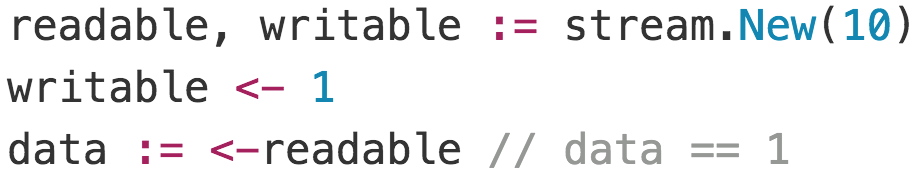
\includegraphics[width=0.55\textwidth]{stream}
  \centering
  \caption{Rivers Stream.}
  \label{code:stream}
\end{figure}

\subsection{Attachables}
\label{sec:rivers:attachable}

Componentes de um pipeline em Rivers precisam satisfazer a interface Attachable \ref{code:rivers:attachable} o que permite com que o contexto de execução atual do componente em questão seja devidamente configurado no momento em que o componente é conectado ao pipeline. É importante que os componentes de um pipeline performem sob um mesmo contexto de execução uma vez que este contexto é usado para sinalizar o término da execução devido a erros ou short-circuit operataions permitindo com que cada componente finalize sua execução apropriadamente.

\begin{figure}[H]
  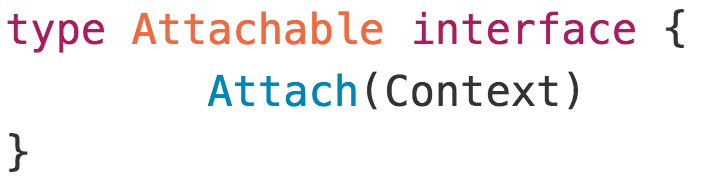
\includegraphics[width=0.4\textwidth]{attachable}
  \centering
  \caption{Attachable Interface.}
  \label{code:rivers:attachable}
\end{figure}

\subsection{Producers}
\label{sec:rivers:producers}

Producers são responsáveis pela produção de dados assincronamente disponibilizando-os em um stream de leitura que é consumido pelo estágio seguinte do pipelinem, aplicando o Pipeline Pattern \ref{subsec:pipeline_pattern}. Para utilizar um tipo como produtor de dados em um pipeline Rivers este deve implementar a interface Producer \ref{code:rivers:producer} do pacote stream, note que um Producer deve satisfazer também a interface Attachable:

\begin{figure}[H]
  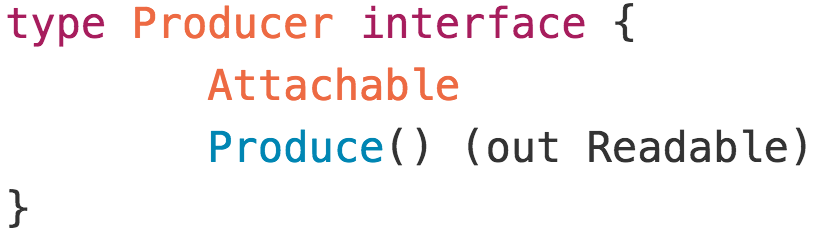
\includegraphics[width=0.45\textwidth]{producer}
  \centering
  \caption{Producer Interface.}
  \label{code:rivers:producer}
\end{figure}

Para que uma implementação de Producer possa ser utilizada em um pipeline Rivers de maneira efetiva, é necessário que o seguinte contrato seja satisfeito:

\begin{enumerate}
  \item Implementar a interface stream.Producer;
  \item Implementar o Pipeline Pattern como parte do método Produce;
  \item Como parte da goroutine produzindo dados: executar em modo defer a função Recover do contexto;
  \item Fechar a componente writable do stream uma vez que a produção de dados é encerrada;
  \item Finalizar a goroutine no caso em que o canal Done ou Failure do contexto forem fechados.
\end{enumerate}

A figura \ref{code:rivers:range_producer} mostra uma implementação de Producer que contempla o contrato anterior, produzindo números inteiros entre um intervalo pré-definido:

\begin{figure}[H]
  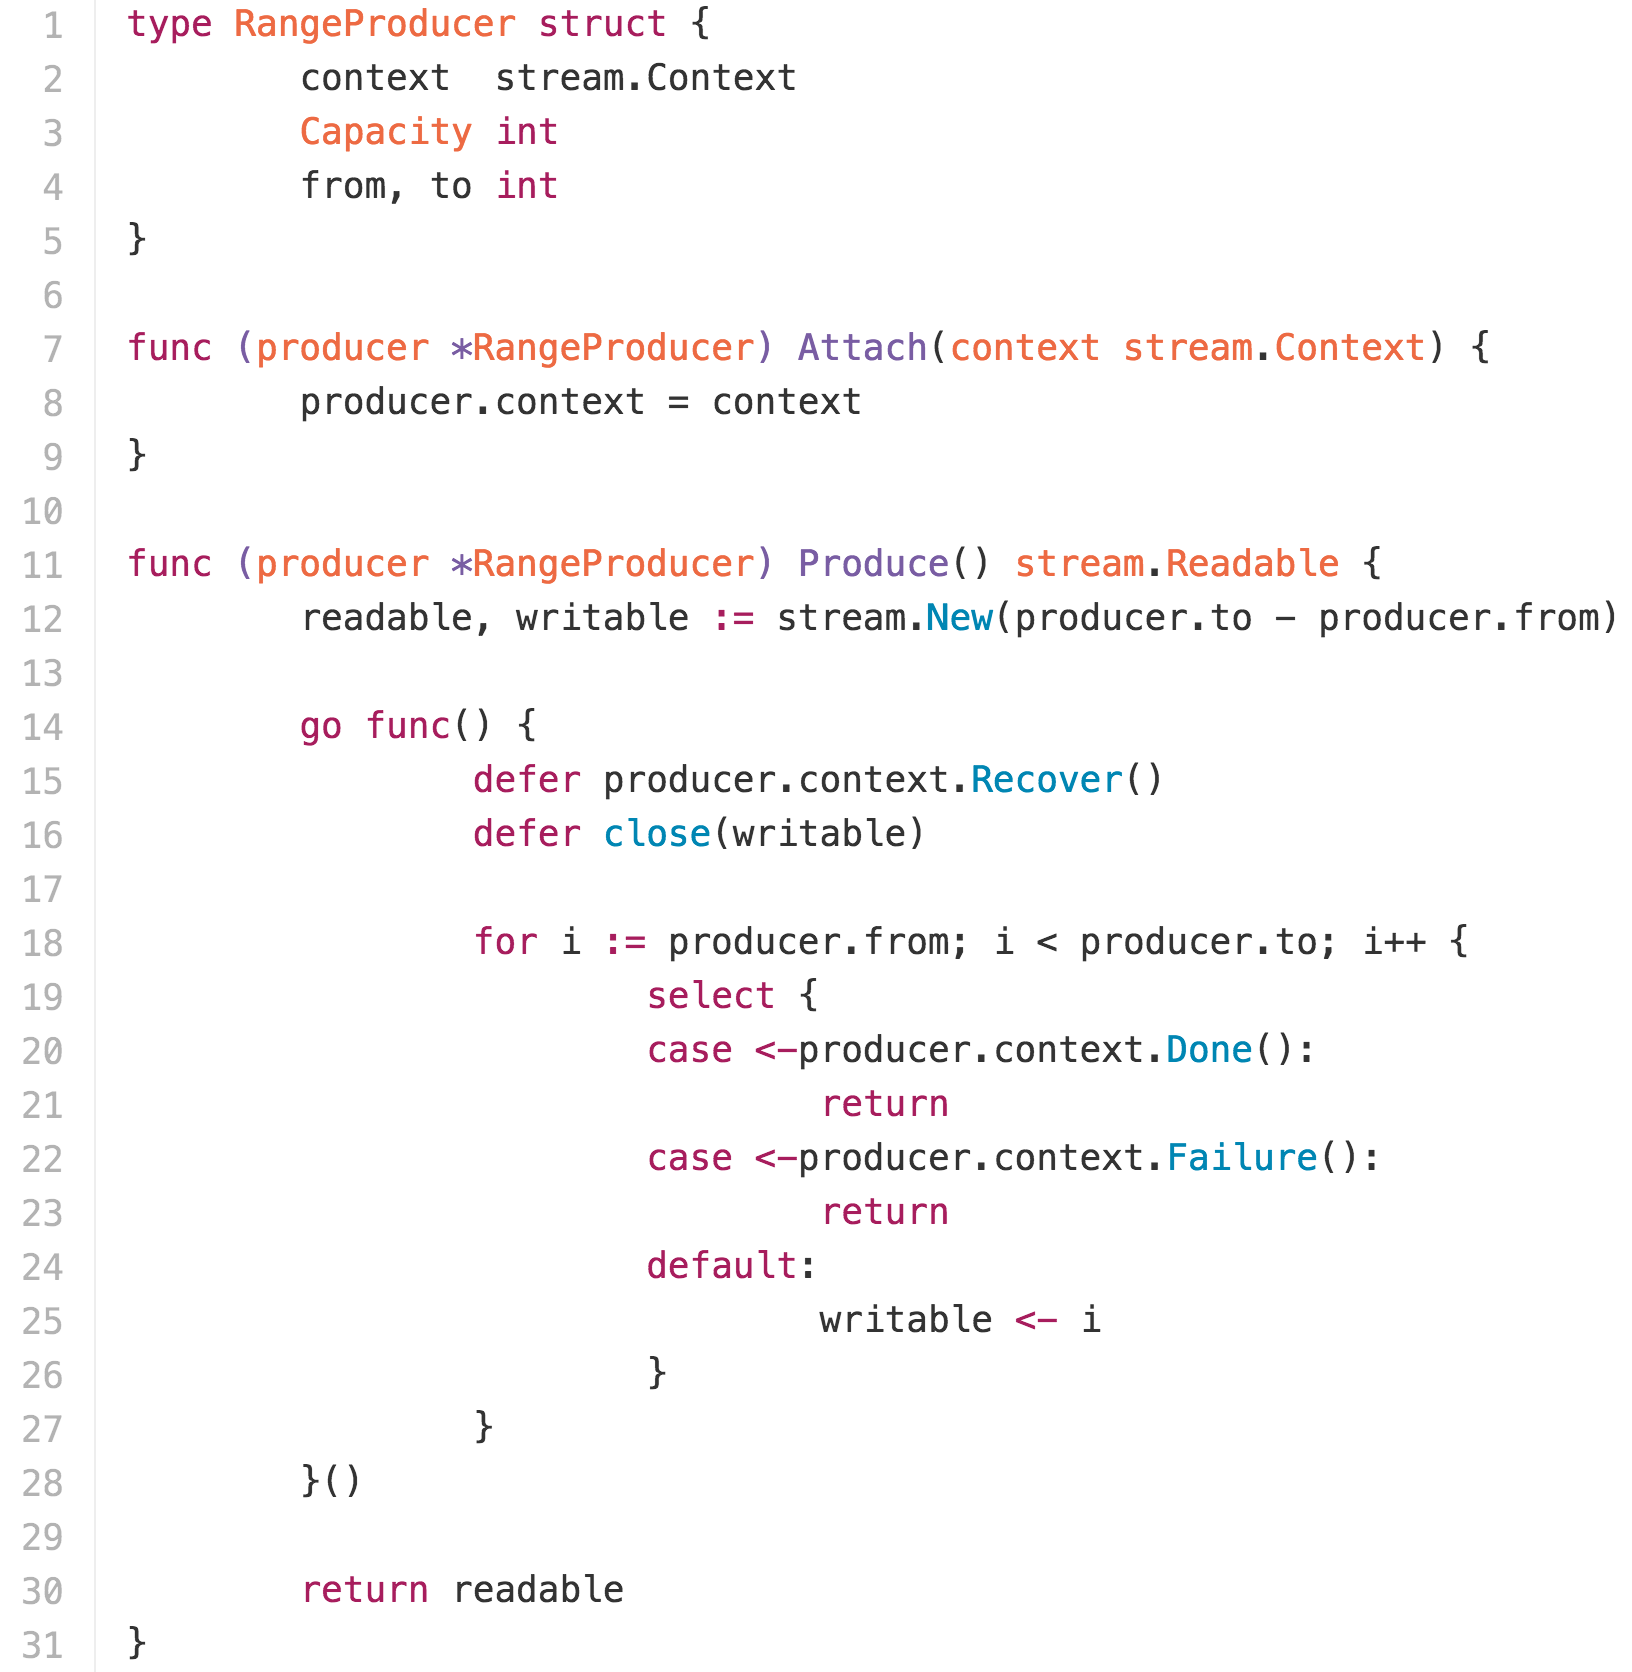
\includegraphics[width=0.95\textwidth]{range_producer}
  \centering
  \caption{Implementação de Producer que gera números inteiros entre um intervalo pré-definido.}
  \label{code:rivers:range_producer}
\end{figure}

Analisando a implementação de RangeProducer é possível verificar que o contrato anterior é implementado corretamente. Cada item do contrato é discutido a seguir:

\begin{enumerate}
\item Implementando os métodos Attach e Produce a interface stream.Producer é satisfeita;
\item O Pipeline Patter é aplicado da seguinte maneira: o método Produce cria um stream na linha 12 com capacidade igual ao quantidade de dados gerados, disparando uma goroutine na linha 14 que assincronamente escreve dados no stream através da componente writable e por fim retorna a componente readable do stream na linha 30 permitindo com que o próximo estágio do pipeline possa eventualmente consumir os dados produzidos.
\item Na linha 15 a função Recover do contexto é executada em modo defer. Isto permite com que o contexto capture e trate qualquer possível erro fatal na execução da goroutine antes que a mesma seja encerrada. Como parte da lógica de Recover, o contexto fecha o canal Failure sinalizando a falha a todos os componentes do pipeline que verificam o estado de falha ao checar o fechamento deste canal em um bloco select, linha 22.
\item Na linha 16 o fechamento da componente writable do stream é executado em modo defer. Esse passo garante que o stream será fechado mesmo em situações de erro fatal ocorridos como parte da execução da goroutine.
\item A execução da goroutine é encerrada caso algum dos canais Done linha 21 ou Failure linha 23 forem fechados. Este mecanismo de parada faz uso de uma propriedade de canais muito importante que diz que todo canal fechado está pronto para receber \ref{subsec:channels} o que faz com que o caso em particular seja selecionado no bloco select. O fechamento do canal Done indica que algum estágio do pipeline requisitou o término da execução por ter finalizado corretamente seu processamento. Esse comportamento pode ser verificado em operações de short-circuit como Find, Any que podem requisitar o término da execução por terem encontrado o resultado o final mesmo que ainda existam dados a serem produzidos. O fechamento do canal Failure por sua vez indica que algum estágio do pipeline encerrou prematuramente devido a uma falha fatal que foi capturada e tratada pela função de Recover do contexto.
\end{enumerate}

Este simples contrato permite com que diversos tipos de Producers sejam criados, simples como o exemplo anterior assim como mais complexos como por exemplo producers que geram dados de um socket, linhas de um arquivo ou até mesmo dados de uma API fornecidos através de um stream HTTP.

Afim de reduzir o boilerplate necessário na implementação de um Producer, Rivers provê o componente Observable do pacote producers que satisfaz por completo o contrato anterior reduzindo consideravelmente o número de linhas necessárias na implementação de um Producer. A implementação de RangeProducer pode ser reescrita em termos de um producers.Observable como mostrado na figura \ref{code:rivers:observable_range_producer}:

\begin{figure}[H]
  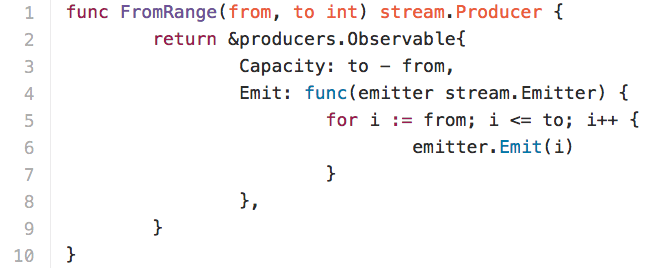
\includegraphics[width=0.8\textwidth]{observable_range_producer}
  \centering
  \caption{Implementação de RangeProducer em termos de producers.Obserbale.}
  \label{code:rivers:observable_range_producer}
\end{figure}

Todos os detalhes do contrato são encapsulados e abstraídos pelo componente Observable. A função Emit linha 4 é executada pelo próprio Observable para dar início o processo de produção dos dados e o componente emitter passado como parâmetro da função é utilizado para emitir os dados produzidos no stream, disponibilizando-os ao próximo estágio do pipeline. Rivers também disponibiliza algumas implementações pré-definidas de producers para processamento de listas, objetos, arquivos e sockets.

\subsection{Transformers}
\label{sec:rivers:transformers}

Transformers são estágios intermediários de um pipeline especializados em transformação de dados. A figura \ref{code:rivers:transformer} mostra a interface implementada por um Transformer.

\begin{figure}[H]
  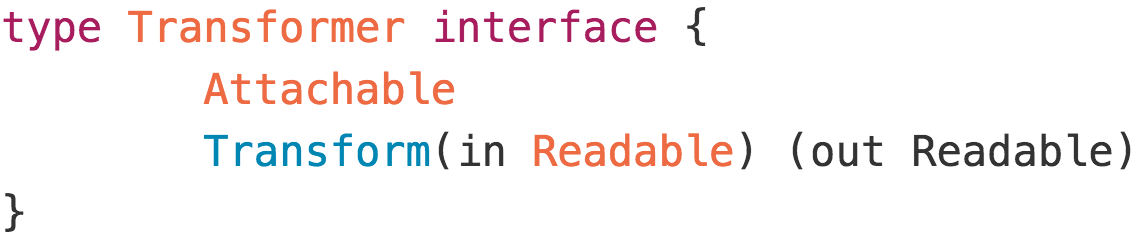
\includegraphics[width=0.6\textwidth]{transformer}
  \centering
  \caption{Transformer Interface.}
  \label{code:rivers:transformer}
\end{figure}

Uma vez conectados à um pipeline, Transformers aplicam sua função de transformação aos dados à medida que passam pelo estágio e seu resultado enviado ao próximo estágio do pipeline. Este processamento é assíncrono e implementado aplicando mais uma vez o Pipeline Pattern.

Em geral transformers são especializados e responsáveis por exercer uma função em específica no contexto de um pipeline. Vários transformers podem ser combinados para realizar lógicas de processamento mais complexas, como por exemplo uma série de filtros seguidos por transformers que acessam dados de uma API, ou banco de dados. Rivers disponibiliza várias funções de transformação pré-definidas como por exemplo Filter, Map, Each e outros.

Implementações de Transformers assim como Producers devem satisfazer um contrato que descreve os pontos necessários que uma implementação deve seguir. Estes pontos são descritos a seguir:

\begin{enumerate}
  \item Implementar a interface stream.Transformer;
  \item Implementar o Pipeline Pattern como parte do método Transform;
  \item Como parte da goroutine transformando dados: executar em modo defer a função Recover do contexto;
  \item Fechar a componente writable do stream uma vez que a transformação de dados é encerrada;
  \item Finalizar a goroutine no caso em que o canal Done ou Failure do contexto forem fechados;
  \item Finalizar a gouroutine caso não haja mais dados a serem consumidos do upstream.
\end{enumerate}

As motivações para cada item do contrato são similares as descritas com relação a implementação de um Producer. A figura \ref{code:rivers:filter_transformer} implementa um Transformer que permite com que apenas números pares sejam enviados ao estágio seguinte do pipeline, e a figura \ref{code:rivers:filter_usage}:

\begin{figure}[H]
  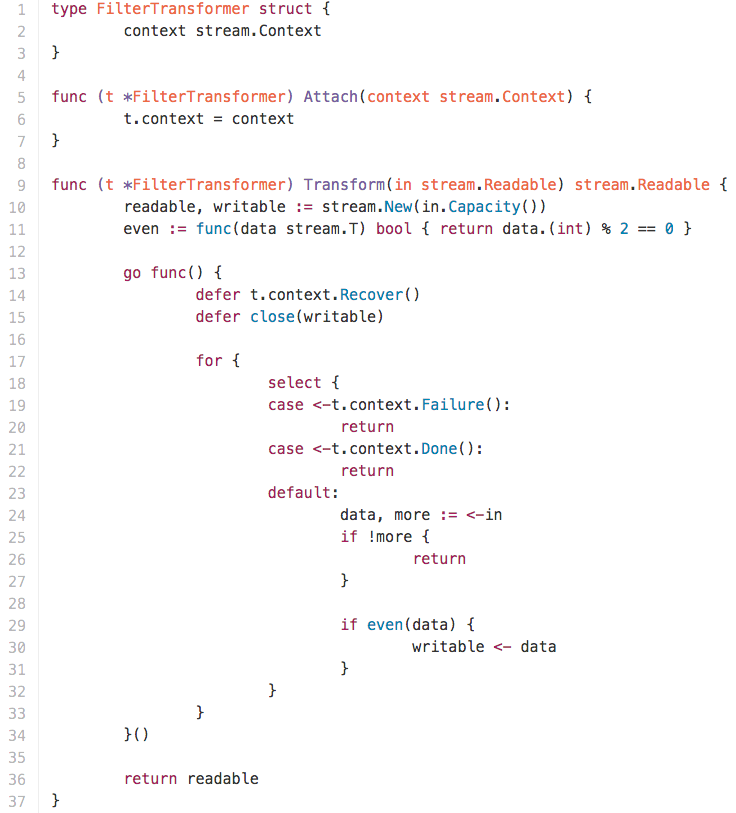
\includegraphics[width=1\textwidth]{filter_transformer}
  \centering
  \caption{Filter Transformer.}
  \label{code:rivers:filter_transformer}
\end{figure}

\begin{figure}[H]
  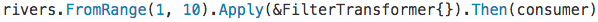
\includegraphics[width=0.85\textwidth]{filter_usage}
  \centering
  \caption{Uso do Filter Transformer em um pipeline Rivers.}
  \label{code:rivers:filter_usage}
\end{figure}

Implementações de transformers e producers são relativamente similares, com algumas restrições:

\begin{enumerate}
  \item Na linha 25 da implementação, a execução do transformer é finalizada caso não existam mais dados a serem consumidos do stream sendo transformado, neste caso o parâmetro in da função Transform;
  \item A operação de filtro é aplicada na linha 29 e dados que satisfazem a condição do filtro, neste caso números pares, são enviados ao estágio seguinte do pipeline.
\end{enumerate}

Rivers disponibiliza o tipo Observer do pacote transformers que encapsula e abstrai cada ponto do contrato mencionado anteriormente e pode ser usado como base da implementação de novos transformers, a figura seguinte reescreve o filtro anterior em termos de um Observer, e seu uso em um pipeline Rivers é mostrado na figura \ref{code:rivers:filter_observer_usage}:

\begin{figure}[H]
  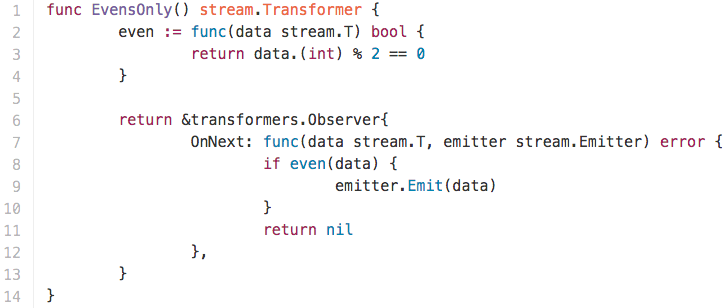
\includegraphics[width=1\textwidth]{filter_observer_transformer}
  \centering
  \caption{Filter Transformer em termos de um Observer}
  \label{code:rivers:filter_observer_transformer}
\end{figure}

\begin{figure}[H]
  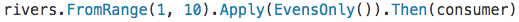
\includegraphics[width=0.75\textwidth]{filter_observer_usage}
  \centering
  \caption{Uso do EvensOnly Filter em um pipeline Rivers.}
  \label{code:rivers:filter_observer_usage}
\end{figure}

Cada dado que chega ao Transformer causa com que o método OnNext do Observer seja invocado com dois parâmetros, o dado em si e uma instância de stream.Emitter que pode ser usado para enviar dados que satisfazem o filtro ao estágio seguinte do pipeline. Caso o método OnNext retorne um erro o pipeline é encerrado e o contexto sinaliza o erro à todos os estágios fechando o channel Failure.

Filtros são operações muito úteis no processamento de streams e são essencialmente especializações de um Transformer. Por este motivo Rivers provê como parte da API mecanismos para se aplicar filtros em um stream de maneira extremamente simples, sem a necessidade de se implementar um novo Transformer. A figura \ref{code:rivers:filters_usage} mostra a aplicação de algumas implementações de filtros existentes na API.

\begin{figure}[H]
  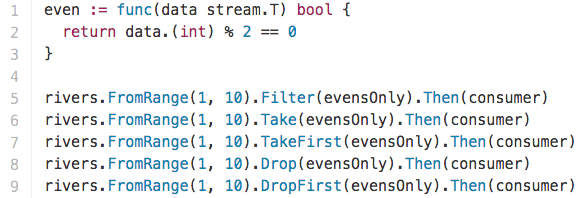
\includegraphics[width=0.85\textwidth]{filters_usage}
  \centering
  \caption{Exemplos de uso de operações de filtros.}
  \label{code:rivers:filters_usage}
\end{figure}

\subsection{Consumers}
\label{sec:rivers:consumers}

Consumers são componentes responsáveis por consumir de maneira síncrona dados de um Readable stream e representam o estágio final do pipeline, eles garantem com que o programa termine apenas ao final da execução do pipeline e reportam qualquer eventual erro de execução do mesmo. Assim como qualquer componente de um pipeline em Rivers, consumers são Attachables podendo ser conectados ao contexto de um pipeline em tempo de execução. A figura \ref{code:rivers:consumer} mostra a interface implementada por um Consumer.

\begin{figure}[H]
  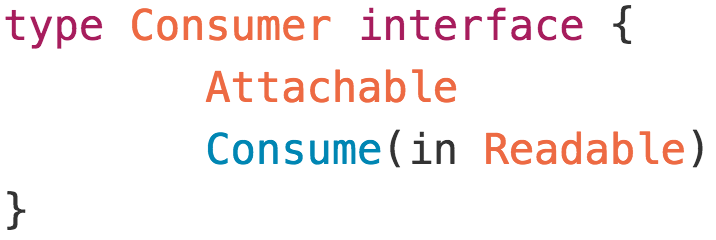
\includegraphics[width=0.35\textwidth]{consumer}
  \centering
  \caption{Consumer Interface.}
  \label{code:rivers:consumer}
\end{figure}

Consumers podem ser utilizados para realizar operações de agregamento de valores como por exemplo Count, que calcula o número total de dados que passam pelo Consumer até o final da execução do pipeline. Outra implementação útil de Consumer são os conhecidos Collectors, componentes responsáveis por coletar os dados que passam pelo consumer para serem utilizados ao final da execução do pipeline. A figura \ref{code:rivers:consumers_usage} mostra algumas aplicações de consumers em Rivers.

\begin{figure}[H]
  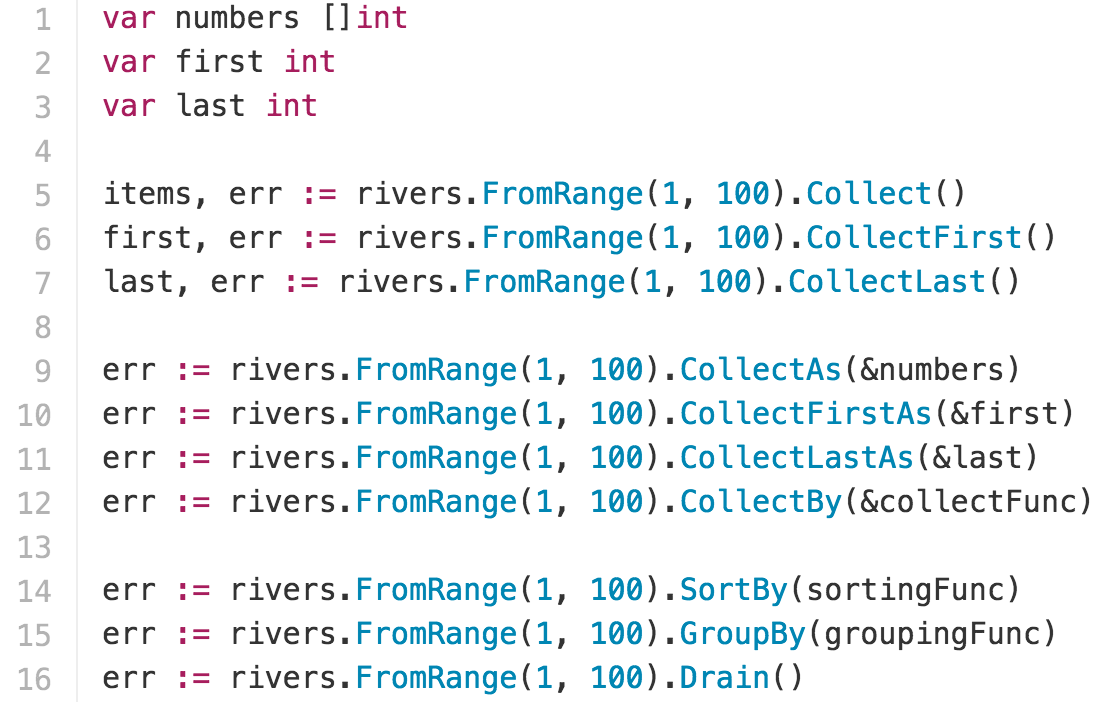
\includegraphics[width=0.75\textwidth]{consumers_usage}
  \centering
  \caption{Aplicação de consumers em Rivers.}
  \label{code:rivers:consumers_usage}
\end{figure}

Consumers ao contrário dos outros componentes do pipeline não implementam o Pipeline Pattern uma vez que estes representam estágios síncronos do pipeline e não produzem stream de dados como resultado. A figura seguir representa uma implementação simples de Consumer que realiza a operação de Count mencionada anteriormente:

\begin{figure}[H]
  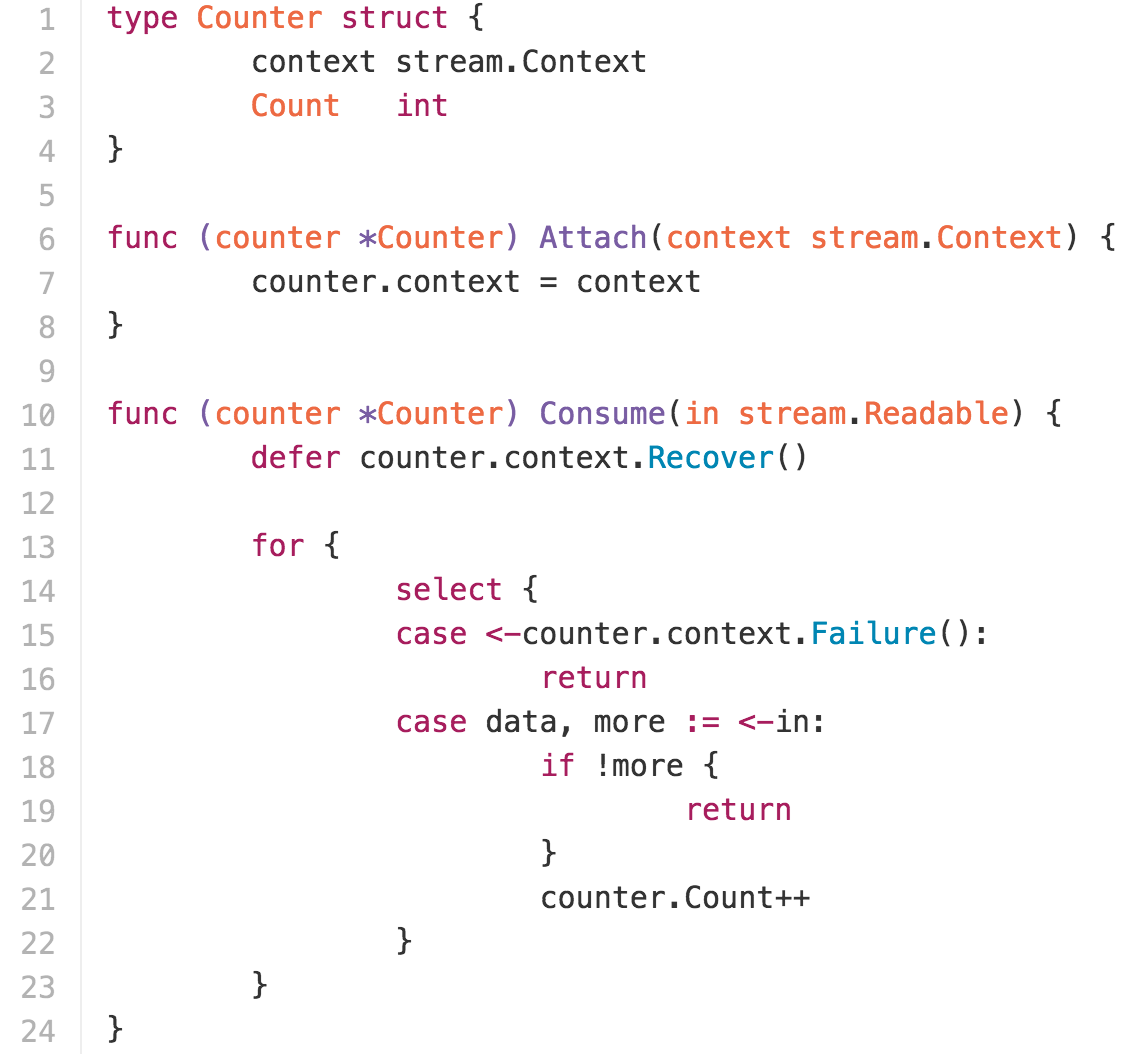
\includegraphics[width=0.75\textwidth]{consumer_count}
  \centering
  \caption{Implementação do Consumer Count.}
  \label{code:rivers:consumer_count}
\end{figure}

O contrato que uma implementação de Consumer deve seguir é relativamente simples, composto por basicamente três passos:

\begin{enumerate}
\item Executar em modo defer a função Recover do contexto como parte da implementação do método Consume;
\item Finalizar a execução caso o canal Failure do contexto foi fechado;
\item Consumir dados do Readable stream até que o stream seja encerrado.
\end{enumerate}

Apesar de simples este contrato acaba por se repetir em diversas implementações de consumers, por isso Rivers disponibiliza o tipo Sink do pacote consumers que pode ser utilizado como base na implementação de novos consumers. A implementação do Consumer Count pode ser reescrita em termos de um tipo Sink como mostrado a seguir:

\begin{figure}[H]
  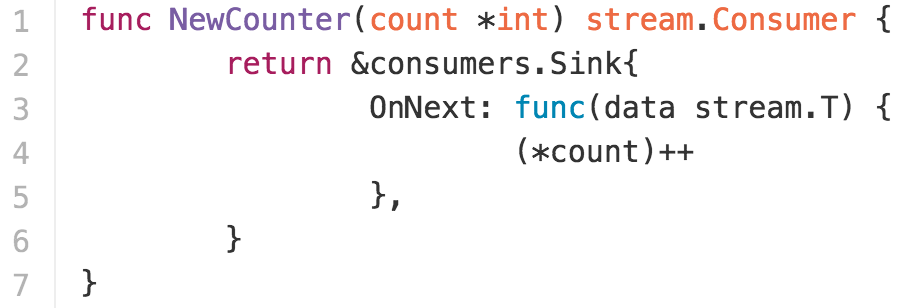
\includegraphics[width=0.6\textwidth]{consumer_count_sink}
  \centering
  \caption{Implementação do Consumer utilizando o tipo Sink como base.}
  \label{code:rivers:consumer_count_sink}
\end{figure}

\subsection{Combiners}
\label{sec:rivers:combiners}

Combiners são mecanismos utilizados para combinar assincronamente diferentes streams de dados em um único stream que pode então ser processado por estágios seguintes do pipeline. Um caso de uso seria combinar diferentes fontes de dados em um único stream, como por exemplo o resultado de uma requisição à uma API restful e uma query à um banco de dados. Os dados produzidos por cada uma dessas fontes de dados após serem combinados em um único Readable stream, podem ser processados pela mesma sequência de estágios. A figura a seguir representa a interface implementada por um Cobiner em Rivers:

\begin{figure}[H]
  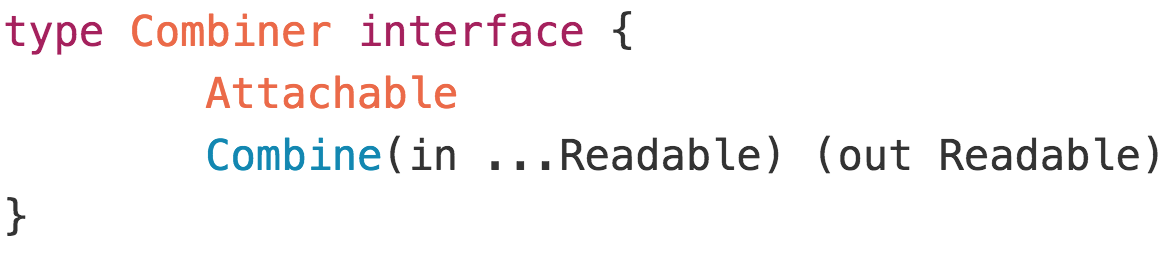
\includegraphics[width=0.6\textwidth]{combiner_interface}
  \centering
  \caption{Combiner Interface.}
  \label{code:rivers:combiner}
\end{figure}

Rivers API além de permitir com que qualquer tipo que satisfaça a interface acima possa ser utilizado como um Combiner em um pipeline, algumas implementações úteis de combiners são nativas da API e prontas para serem utilizadas como por exemplo Merge que combina dados de fontes diferentes em uma política FIFO aonde os primeiros dados que chegam de qualquer uma das fontes são imediatamente enviados para o stream final. Outra política de junção de streams é a de Zip que coleta um item de cada fonte alternadamente até que todos os dados sejam combinados, dentre outras implementações.

\begin{figure}[H]
  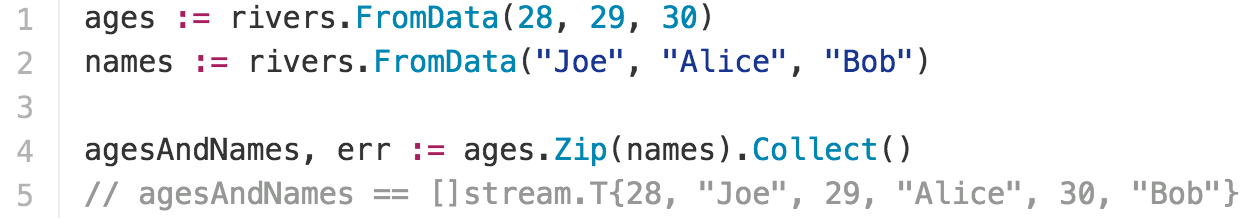
\includegraphics[width=0.9\textwidth]{zip_combiner}
  \centering
  \caption{Zip Combiner Interface.}
  \label{code:rivers:zip_combiner}
\end{figure}

\subsection{Dispatchers}
\label{sec:rivers:dispatchers}

Dispatchers são utilizados para assincronamente redirecionar o fluxo de dados de um Readable stream à um ou mais Writable streams particionando o pipeline em vários ramos. Em casos mais complexos, Dispatchers podem implementar diferentes lógicas de redirecionamento utilizando funções de classificação conhecidas como predicados, nestes casos os dados que não satisfazerem o predicado são redirecionados a um Readable stream resultante da operação. A figura \ref{code:rivers:dispatcher} representa a interface implementada por um Dispatcher.

\begin{figure}[H]
  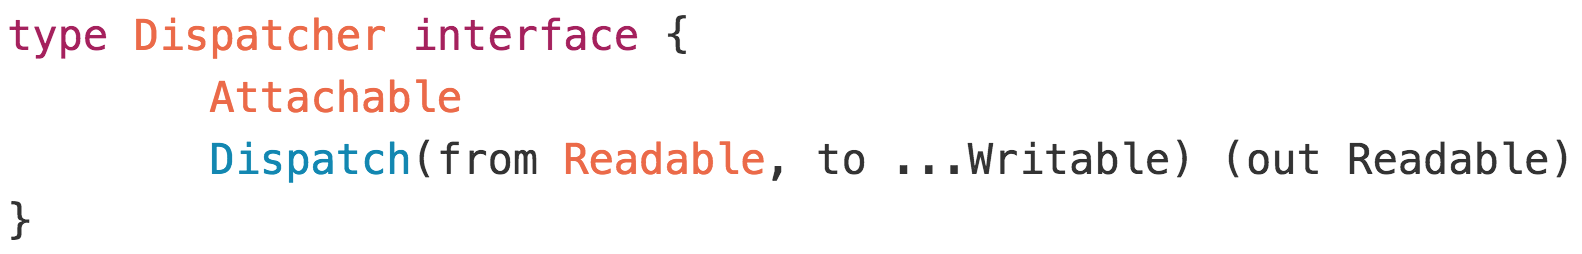
\includegraphics[width=0.85\textwidth]{dispatcher_interface}
  \centering
  \caption{Dispatcher Interface.}
  \label{code:rivers:dispatcher}
\end{figure}

Em particular dispatchers são úteis para classificar e agrupar dados em streams diferentes podendo processar cada stream utilizando lógicas específicas. Operações de partição são exemplos clássicos de Dispatchers em Rivers. A figura a seguir mostra um stream de números inteiros sendo particionado em dois outros streams, o primeiro contendo apenas números pares e o segundo números ímpares.

\begin{figure}[H]
  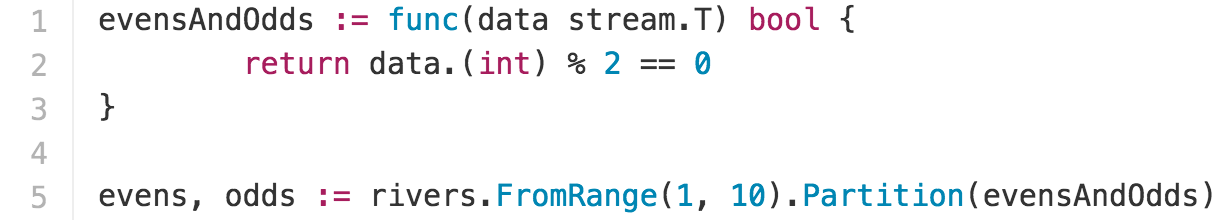
\includegraphics[width=0.85\textwidth]{partition_dispatcher}
  \centering
  \caption{Exemplo de particionamento de um stream de números inteiros.}
  \label{code:rivers:partition_dispatcher}
\end{figure}

Rivers API disponibiliza algumas implementações de dispatchers pré-definidas além da mencionanda anteriormente, como por exmplo Split que duplica um stream em dois outros idênticos útil para aplicar diferentes sequências de transformações concorrentes aos dados do stream como por exemplo salvar entidades na base de dados e concorrentemente indexar a informação em uma engine de busca ou salvar a informação em uma cache.

\subsection{O Contexto Global}
\label{sec:rivers:context}

Coordenar vários estágios concorrentes de um pipeline e garantir o término da execução mesmo na presença de erros são algumas das funções do contexto o qual é compartilhado por cada componente conectado ao pipeline. Um contexto implementa alguns mecanismos utilizados por cada componente descrito até o momento que permitem com que cada um deles possam sinalizar o término da execução devido a uma falha por exemplo, permitindo com que qualquer goroutine em execução possa suspender seu processamento verificando o canal Failure do contexto. Em casos em que um estágio do pipeline falhe causando uma situação de panic, o programa não finaliza inesperadamente uma vez que como descrito nos contratos de cada componente, a função de Recover do contexto é executada em modo defer como parte do processamento permitindo que o contexto capture o erro e sinalize a falha fechando o canal Failure causando com que cada componente suspenda sua execução liberando qualquer recurso de máquina utilizando até o momento, como conexões com base de dados, descritores de arquivos, etc.

\begin{figure}[H]
  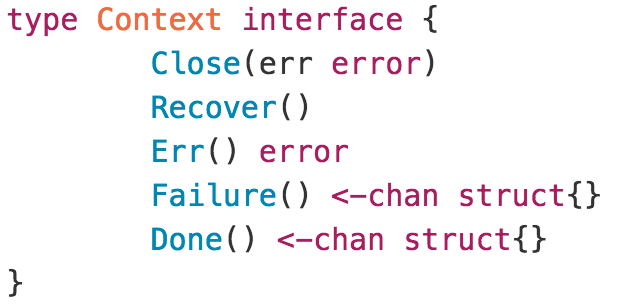
\includegraphics[width=0.45\textwidth]{context}
  \centering
  \caption{Context Interface.}
  \label{code:rivers:context}
\end{figure}

A figura acima representa a interface implementada por um contexto em Rivers. Qualquer componente conectado ao pipeline pode verificar o estado atual do pipeline através dos canais de comunicação Failure e Done do contexto ou requisitar o término da execução através do método Close de um contexto, provendo uma informação de erro opcional. Caso nenhum erro seja fornecido, a execução do pipeline é finalizada com sucesso mesmo que ainda haja elementos a serem produzidos. Este cenário é usual em operações de short-circuit como Find que sinaliza o término do pipeline assim que o primeiro elemento satisfazendo a condição de busca passe pelo estágio.

Em casos em que o canal Done do contexto é fechado qualquer Producer ou Transformer conectados ao pipeline de acordo com seus contratos devem encerrar seus processamentos liberando qualquer recurso alocado durante sua execução. Este mecanismo aonde cada componente é responsável por verificar o estado atual do contexto antes de realizar qualquer processamento e suspender a execução em caso de término devido a erros -- canal Failure -- ou devido ao término prematuro -- canal Done -- permite com que centenas de milhares de estágios concorrentes sejam conectados ao pipeline sem impactar na complexidade de gerência e coordenamento do pipeline, uma vez que sinalizar o término da execução de cada um destes estágios se resume no fechamento de um dos canais mencionados. Isso é possível devido ao excelente modelo de concorrência da linguagem Go que baseia-se na filosofia de compartilhamento de memória através da comunicação em vez de comunicar através do compartilhamento de memória.

\section{Suporte a Paralelização}
\label{sec:rivers:going_parallel}

Concorrência e paralelismo são conceitos similares porém diferentes, assim como abordado de maneira brilhante por Rob Pike em sua talk \cite{talk:rob_pike:concurrency_not_parallelism} Concurrency is not Parallelism. Estágios de um pipelines em Rivers são processados concorrentemente e cada estágio pode ainda ser paralelizado utilizando os recursos de hardware como multi-cores para atingir níveis extremos de paralelismo aumentado a eficiência do pipeline.

Rivers permite que certos tipos de Transformers possam ser paralelizados, como por exemplo um Map ou Each Transformer. Para atingir níveis aceitáveis de paralelismo Rivers replica o Transformer em questão em vários outros, tantos quanto for a capacidade do stream sendo consumido, por exemplo se um producer tem a capacidade de produção de 3 elementos o Transdormer seria replicado obtendo 3 instâncias paralelas. Cada novo Trnasformer consome dados do estágio anterior concorrentemente, produzindo seus resultados em um mesmo stream resultante que é consumido pelo estágio senguinte do pipeline. A figura \ref{fig:rivers:rivers_parallel} mostra como seria o fluxo de um pipeline com paralelismo ativado.

\begin{figure}[H]
  \includegraphics[width=0.55\textwidth]{rivers_parallel}
  \centering
  \caption{Fluxo de um Pipeline com Paralelismo ativado.}
  \label{fig:rivers:rivers_parallel}
\end{figure}

Essa solução permite aliviar bottlenecks relacionados a estes tipos de Transformers. O código \ref{code:rivers:parallel_pipeline} mostra um exemplo de pipeline sendo executado sequencialmente e outro com paralelismo ativado:

\begin{figure}[H]
  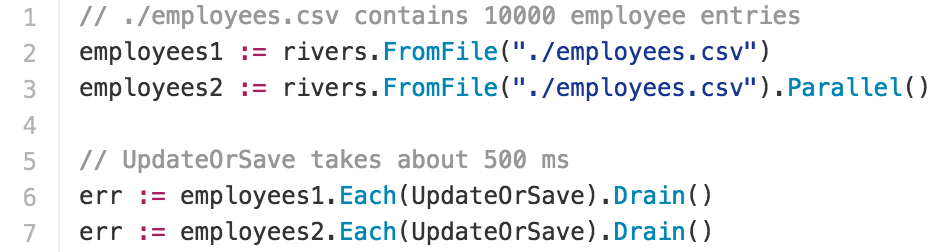
\includegraphics[width=0.8\textwidth]{parallel_pipeline}
  \centering
  \caption{Exemplo de Paralelismo em Rivers.}
  \label{code:rivers:parallel_pipeline}
\end{figure}

No exemplo acima, dois pipelines são criados para processar um arquivo CSV contendo 10000 entradas com informações de empregados de uma determinada empresa. Para cada empregado deve-se verificar sua existência na base de dados atualizar determinada informação caso exista, ou criar uma nova entrada para o empregado correspondente. Esse procedimento leva em torno de 500 ms por empregado. O primeiro pipeline por não utilizar paralelismo levaria um tempo total de aproximadamente 1.38 horas para finalizar o processamento. Já o segundo pipeline, por ativar o uso de paralelismo, Rivers replica o estágio Each para cada entrada de Employee extraída do arquivo CSV executando cada estágio concorrentemente distribuindo a carga de trabalho em diferentes threads fazendo o uso de todos os cores disponíveis na máquina. O tempo total de execução do segundo pipeline medido em uma máguina com 8 cores foi de aproximadamente 2.58 segundos.

\chapter{Processo de Desenvolvimento}
\label{cha:rivers_implementation}

Rivers surgiu da necessidade de se implementar soluções simples porém eficientes para o processamento de grandes volumes de dados. Na empresa Bearch Inc esse processo é recorrente e pela falta de uma solução nativa no contexto da linguagem de programação Go utilizada amplamente nos projetos internos da empresa, desenvolvedores acabavam por implementar lógicas de processamento redundantes que se repetiam ao longo do desenvolvimento de vários projetos. Devido aos custos deste retrabalho e aos padrões encontrados no processo de desenvolvimento de vários projetos, foi proposto uma solução para ajudar a reduzir a quantidade de código necessário para se implementar essas rotinas de processamento assim como possibilitar o reuso de lógicas existentes de soluções anteriores.

Este capítulo discute brevemente o processo de desenvolvimento empregado assim como as práticas utilizadas para guiar a evolução da solução minimizando a quantidade de retrabalho necessário ao longo das iterações.

\section{Coleta de Requisitos e Roadmap}
\label{sec:requirements}

Requisitos foram levantados afim de se ter um conjunto mínimo de funcionalidades que pudesse formar o MVP inicial para que se iniciasse o desenvolvimento. A tabela \ref{mvp:requirements} lista as features consideranas no Roadmap de Rivers, algumas delas selecionadas para compor o MVP e outras implementadas somente na versão seguinte. As features marcadas para compor o MVP foram selecionadas com o intuito de se ter o mínimo de funcionalidades disponíveis para se implementar um pipeline de processamento de streams que possa ser utilizado em diferentes contextos já identificados em projetos anteriores da empresa, como por exemplo no processamento de entidades da base de dados assim como no processamento de resultados de chamadas de APIs de outros sistemas.

\begin{table}[h!]
    \centering
    \begin{tabular}{||c c c||} 
        \hline
        Backlog & MVP & V2.0 \\ [0.5ex] 
        \hline\hline
        Contexto Global & X & \\ 
        \hline
        Producer Interface & X & \\ 
        \hline
        Producers Especializados (List, Socket, File...) & & X \\ 
        \hline
        Transformer Interface & X & \\ 
        \hline
        Transformers Especializados (Map, Each, Filter...) & & X \\ 
        \hline
        Consumer Interface & X & \\
        \hline
        Consumers Especializados (Count, Reduce...) & & X \\
        \hline
        Dispatchers & & X \\
        \hline
        Combiners & & X \\
        \hline
        Panic Recovering & X & \\
        \hline
        Failure Retries & & X \\
        \hline
        Suporte a Paralelização & & X \\
        \hline
        Pipelines Distribuídos & & X \\ [1ex]
        \hline
    \end{tabular}
    \caption{Rivers Roadmap: MVP vs. V2.0}
    \label{mvp:requirements}
\end{table}

Afim de atender as necessidades dos projetos utilizados como casos de uso, foi decidido então que uma solução útil e viável teria que prover pelo menos uma implementação genérica de cada um dos estágios que compõem um pipeline. Um Producer deveria permitir com que diferentes fontes de dados sejam utilizadas no pipeline como geradores de dados como por exemplo base de dados, APIs Restful e arquivos. Uma implementação de Transformer deve permitir que uma lógica específica de processamento possa ser aplicada aos dados sendo transmitidos pelo stream e seu resultado passado ao próximo estágio. Um Consumer por sua vez deve permitir que dados possam ser coletados de maneira síncrona ao final do pipeline assim como possíveis erros de execução. Por fim, a implementação inicial deveria prover um mecanismo simples que pudesse detectar falhas em tempo de execução notificando-as aos estágios do pipeline para que os mesmos possam suspender sua execução.  Implementações mais especializadas de cada um destes estágios seriam o foco em versões futuras da API como por exemplo producers especializados em leitura de arquivos, drivers de base de dados específicas, transformers especializados em operações como Map, Reduce, Filter, etc, mecanismos para se executar o pipeline de maneira distribuída em um cluster de máquinas.

O plano de desenvolvimento foi mantido e disponibilizado como GitHub \ref{github} issues apresentado através de um dashboard Kanban \ref{kanban} disponível em Waffle.io \ref{waffle} para facilitar a visualização do progresso mantendo a informação e comunicação centralizada, como mostrado na figura \ref{fig:waffle}. Ao longo do desenvolvimento, cada feature implementada era prontamente testada em casos de uso reais por outros desenvolvedores e feedbacks coletados afim de aprimorar a solução de acordo com as necessidades reais do time.

\begin{figure}[H]
  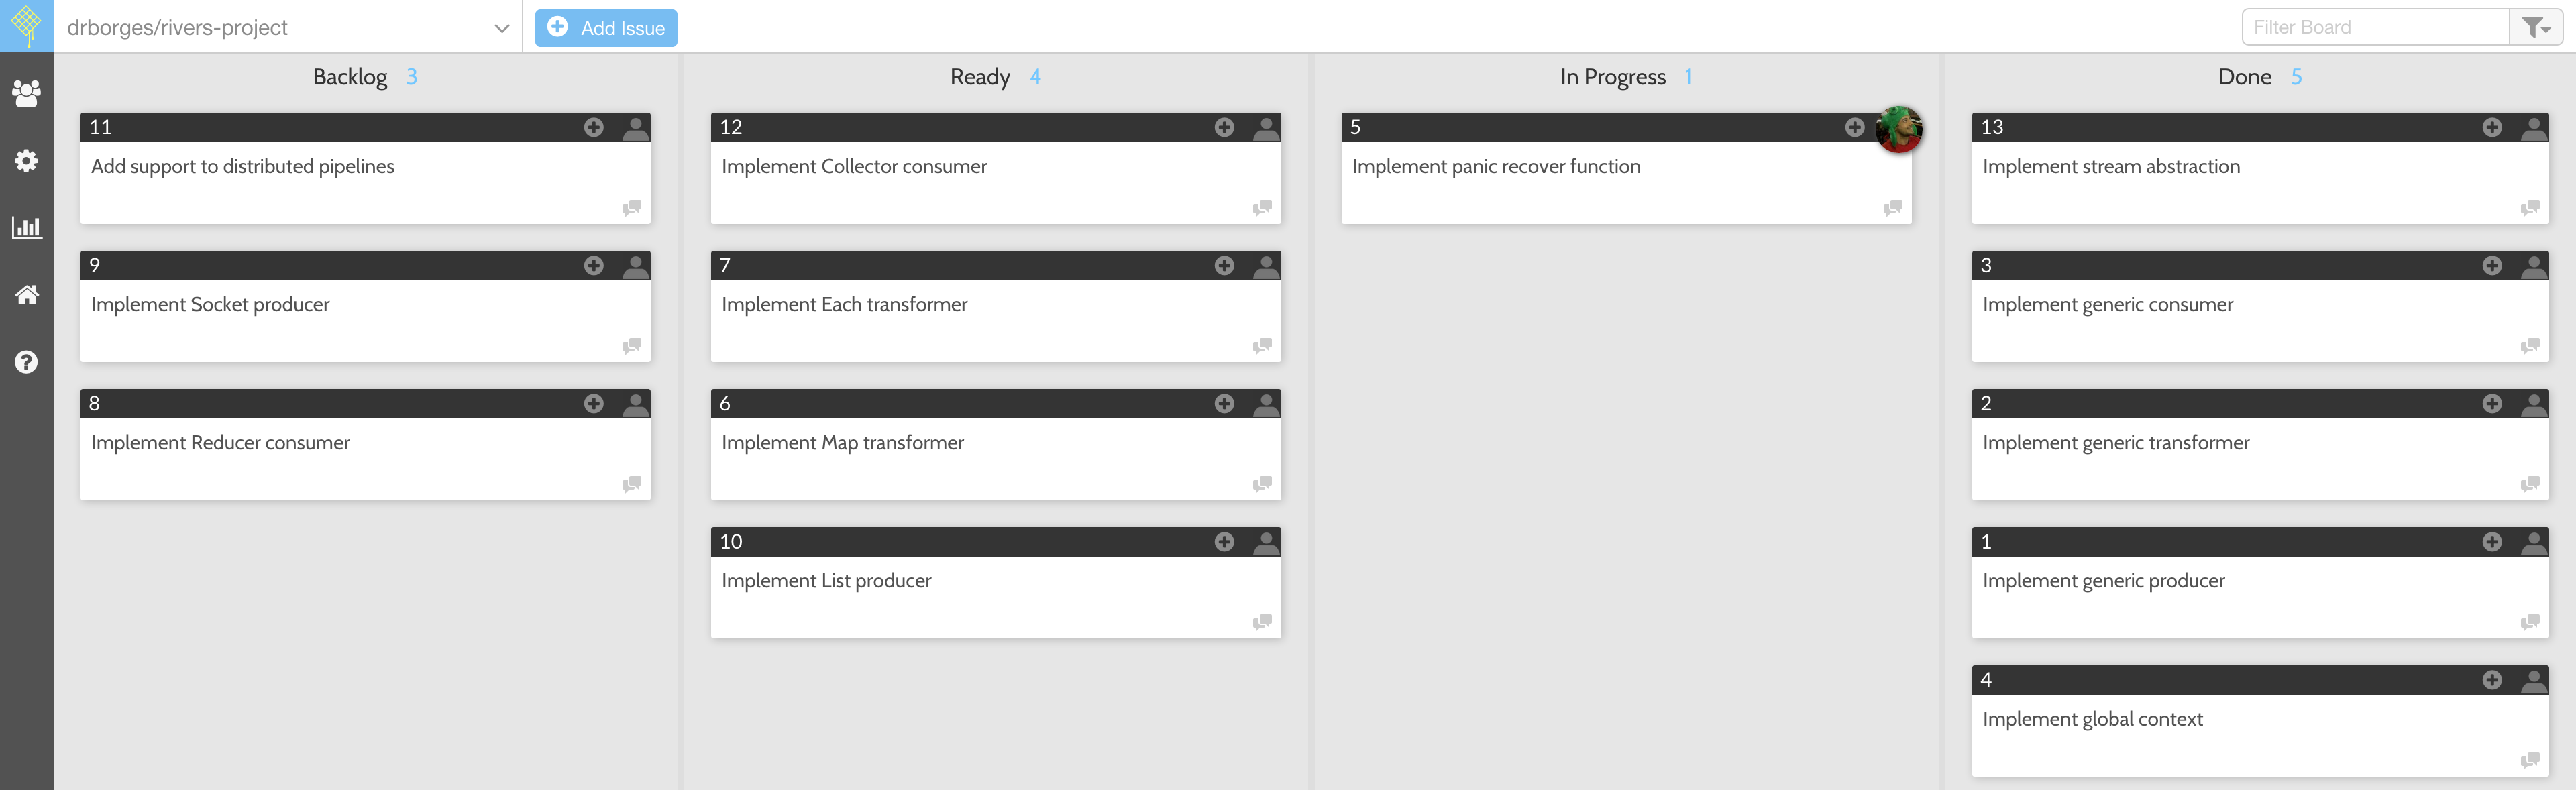
\includegraphics[width=1\textwidth]{waffle}
  \centering
  \caption{Roadmap visualizado em um dashboard Waffle.}
  \label{fig:waffle}
\end{figure}

\section{Tests \& Benchmarks}
\label{sec:tests_n_benchmarks}

Foi utilizada a técnica Test Driven Development \cite{book:tdd:kent_beck} para toda nova funcionalidade implementada. Escrevendo-se os casos de teste antes mesmo de se ter a funcionalidade ajudou a guiar o design da API gradativamente, uma vez que toda complexidade envolvida na implementação da nova funcionalidade era colocado inicialmente de lado, permitindo o desenvolvedor focar no design da API se colocando como usuário da mesma em um primeiro momento. Através do uso desta técnica, foi possível alcançar uma cobertura de testes razoável criando um conjunto de testes de regressão muito útil na detecção de quebra de funcionalidades já existentes devido a alterações de certas áreas do codebase. Visando tirar o máximo de proveito da técnica, foi utilizado a ferramenta fsnotify \cite{tools:fsnotify} para execução dos testes de regressão sempre que um arquivo no codebase é alterado, disponibilizando um relatório dos resultados de cada teste executado com isso um feedback instantâneo com relação as últimas alterações no codebase. A figura \ref{fig:tdd-cycle} representa o ciclo de desenvolvimento seguido aplicando a técnica TDD.

\begin{figure}[H]
  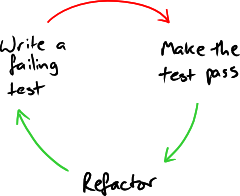
\includegraphics[width=0.4\textwidth]{tdd-cycle}
  \centering
  \caption{Ciclo de desenvolvimento aplicando a técnica TDD.}
  \label{fig:tdd-cycle}
\end{figure}

Alguns benchmarks foram implementados para medir a eficiência de um pipeline segundo a solução proposta em comparação com soluções utilizada previamente em outros projetos. A tabela a seguir mostra os resultados medidos entre duas versões de um Job que processa 1000 entidades datastore por vez aonde o processamento leva em média 1 seg por entidade. Em uma versão foi implementado um pipeline Rivers com paralelização ativada afim de tirar o máximo de proveito do hardware utilizado. A outra implementação segue uma solução sequencial utilizada anteriormente em outros projetos.

\begin{table}[h!]
    \centering
    \begin{tabular}{||c c c||} 
        \hline
        Jobs & Número de Goroutines & Tempo Médio de Execução (seg) \\ [0.5ex] 
        \hline\hline
        Pipeline Rivers & 1000 & 1.16 \\ 
        \hline
        Solução Sequencial & 1 & >1000 \\ [1ex]
        \hline
    \end{tabular}
    \caption{Comparação entre Jobs sequencial e Rivers paralelizado}
    \label{benchmarks:sequential_vs_parallel}
\end{table}

\chapter{Rivers: Applicações Reais}
\label{cha:applications}

\section{Appx - Appengine eXtensions}
\label{sec:appx}

\emph{Appx} \cite{docs:drborges:appx} é um conjunto de extensões da plataforma \emph{Appengine} da Google \cite{docs:google:appengine} para o runtime da linguagem Go que oferece uma solução similar à Object Relational Mapping \cite{article:scott:orm} para modelagem da camada de domínio de aplicações que utilizam a solução de \emph{NoSQL} \cite{article:fowler:nosql} Datastore \cite{docs:google:datastore} da plataforma. Rivers foi utilizado para dar suporte à \emph{Continuous Querying Over Data Stream} \cite{paper:badu:continuous_querying}, permitindo que grandes conjuntos de dados possam ser continuamente buscados da base de dados em batches via paginação e processados assincronamente como um stream de entidades Datastore em poucas linhas de código.

Processar um grande conjunto de dados aplicando filtros, mapeamentos e realizando a paginação dos resultados é relativamente complexo quando se utilizando apenas as APIs nativas do Datastore. Desenvolvedores precisam explicitamente implementar a paginação contínua dos dados através da manipulação de cursores de busca, realizar tratamento de possíveis erros de execução além de implementar a lógica de processamento dos dados, sendo necessário várias linhas de código para se obter o resultado final levando a uma solução difícil de manter e muita duplicação de código quando esse processamento deve ser aplicado à diferentes entidades da base de dados. A figura \ref{code:datastore:pagination} mostra a implementação de um agendador de reuniões que envia email, sms e atualiza o calendário de cada empregado de uma empresa cujo título seja \emph{Manager} ou \emph{Director} com as informações da reunião. Devido a uma limitação do Datastore, é possível processar no máximo 1000 entidades por vez, sendo necessário realizar a paginação contínua dos dados até que todos eles sejam processados. Grande parte desta implementação não possui relação direta com a lógica necessária para o agendamento da reunião mas sim com a paginação dos dados.

\begin{figure}[H]
  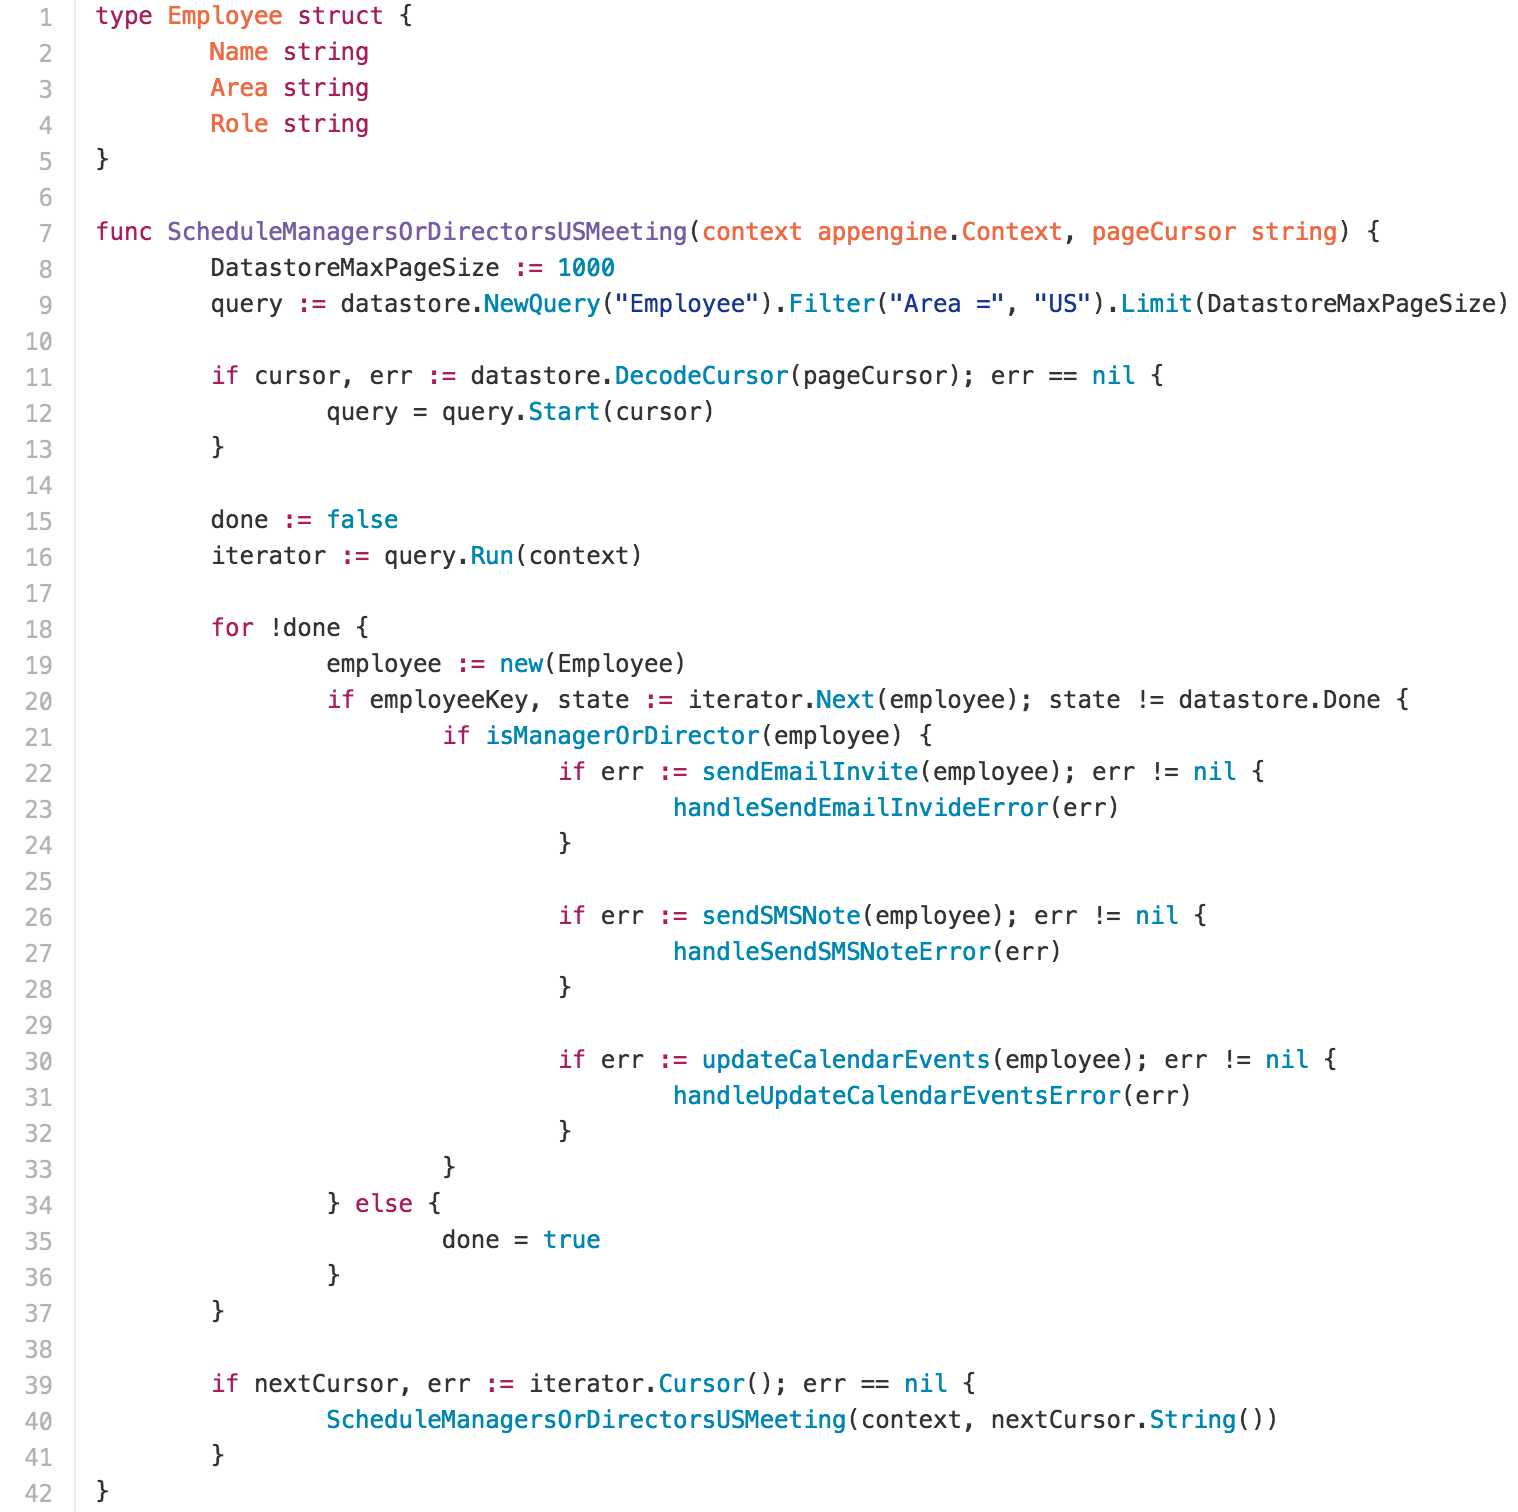
\includegraphics[width=1\textwidth]{datastore_pagination}
  \centering
  \caption{Exemplo de uso da API nativa do Datastore.}
  \label{code:datastore:pagination}
\end{figure}

Appx utiliza Rivers para reduzir grande parte desta complexidade sendo necessárias poucas linhas de código para se obter o mesmo resultado do exemplo anterior. A figura \ref{code:appx:stream} mostra como podemos reescrever este mesmo caso de uso utilizando a API de streamming de Appx. Devido à arquitetura extensível de Rivers sua integração com Appx é relativamente simples, sendo necessário que Appx apenas implemente a interface \emph{stream.Producer} de Rivers que encapsula a execução da query, tratamento de erros e a paginação contínua dos resultados emitindo cada entidade datastore que satisfaz a query em um \emph{stream.Readable} ao qual operações como \emph{Filter}, \emph{Each}, \emph{Map} e \emph{Reduce} podem ser aplicadas formando um pipeline de processamento de entidades \emph{Datastore}. Desta maneira o resultado final não é somente mais legível mas como também fácil de manter e alterações na lógica de processamento é tão simples como adicionar ou remover filters, mappers, etc. 

\begin{figure}[H]
  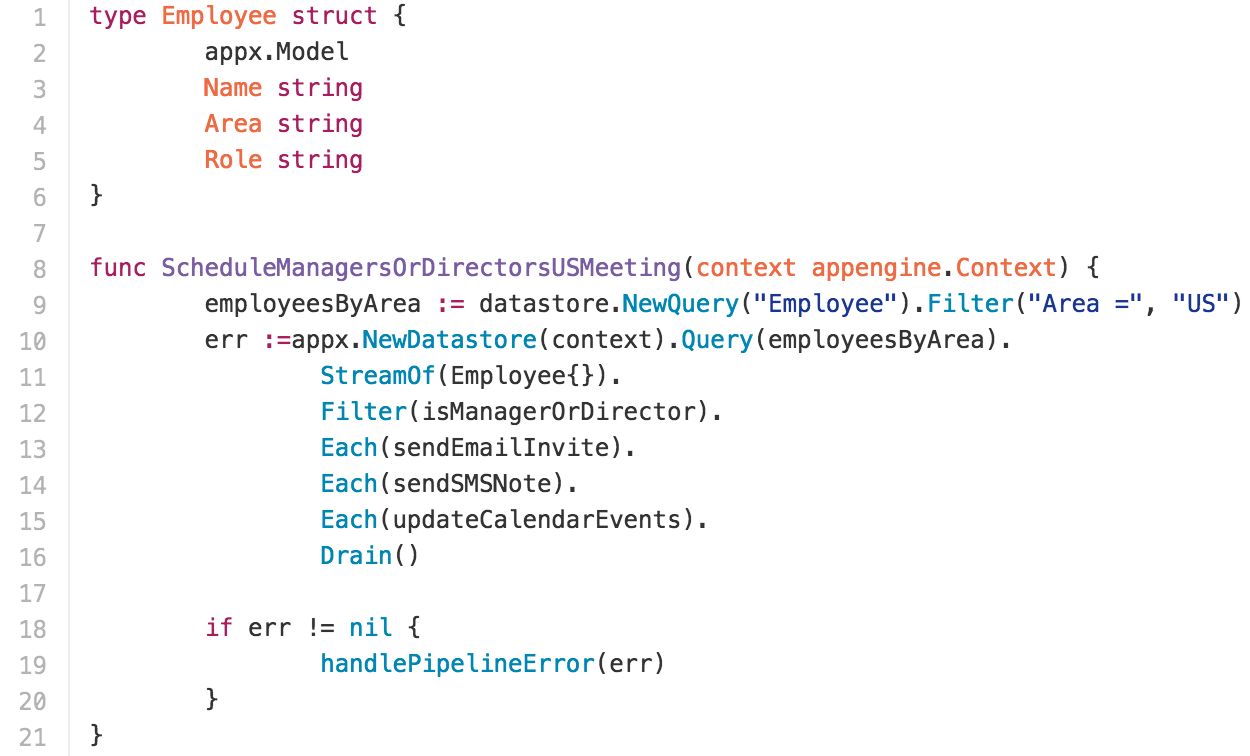
\includegraphics[width=1\textwidth]{appx_stream}
  \centering
  \caption{Exemplo de uso da API de streamming do framework Appx.}
  \label{code:appx:stream}
\end{figure}

\section{Web Scrapping}
\label{sec:web_scrapping}

Web Scraping \cite{article:webharvy:scrapping} é uma solução simples, barata e eficaz para coleta e extração de dados na web e frequentemente são aplicados em conjunto com \emph{Web Crawlers} \cite{article:howstuffworks:web_crawler}, sistemas responsáveis por automatizar a busca e descoberta da informação, basicamente acessando documentos web através de \emph{URLs}, coletando e visitando cada URL no documento retornado aplicando este processo recursivamente até que uma determinada condição de parada seja satisfeita, afim de extrair e agregar determinados tipos de informação presentes em cada documento.

Este processo de crawling por envolver altos níveis de tráfego de rede pode vir a ser muito custoso e a possibilidade de paralelizar partes do processo pode ajudar a reduzir este custo. Rivers pode ser utilizado na implementação de pipelines com foco em Web Crawling e Scrapping, aonde cada crawler implementa a interface \emph{stream.Producer} com uma lógica específica responsável por "caminhar" a web seguindo determinadas regras específicas do crawler passando cada documento encontrado ao próximo estágio do pipeline que implementa a interface \emph{stream.Transformer} responsável por extrair as informações necessárias do documento implementando a função de scrapping. A imagen \ref{code:crawler} mostra um exemplo de Crawler utilizado como \emph{stream.Producer} em um pipeline Rivers responsável por extrair URLs de documentos HTML com a listagem de gastos públicos das cidades do Rio Grande do Sul disponíveis no \cite{portal_transparencia}, passando cada URL ao estágio seguinte do pipeline que implementa um scrapper \ref{code:scrapper} que dado uma URL o documento correspondente é recuperado via HTTP e as informações de gastos extraídas e coletadas em um dicionário chave-valor aonde a chave representa a área correspondente ao gasto como por exemplo educação ou saúde, e seu valor o total investido nesta área. A figura \ref{code:scrapping_example} mostra o uso do Crawler e Scrapper em um pipeline Rivers com paralelização ativa, podendo processar até 510 URLs em paralelo que é o número total de cidades a serem processadas e representa a capacidade máxima de produção do pipeline especificado pelo Crawler na linha 25.

\begin{figure}[H]
  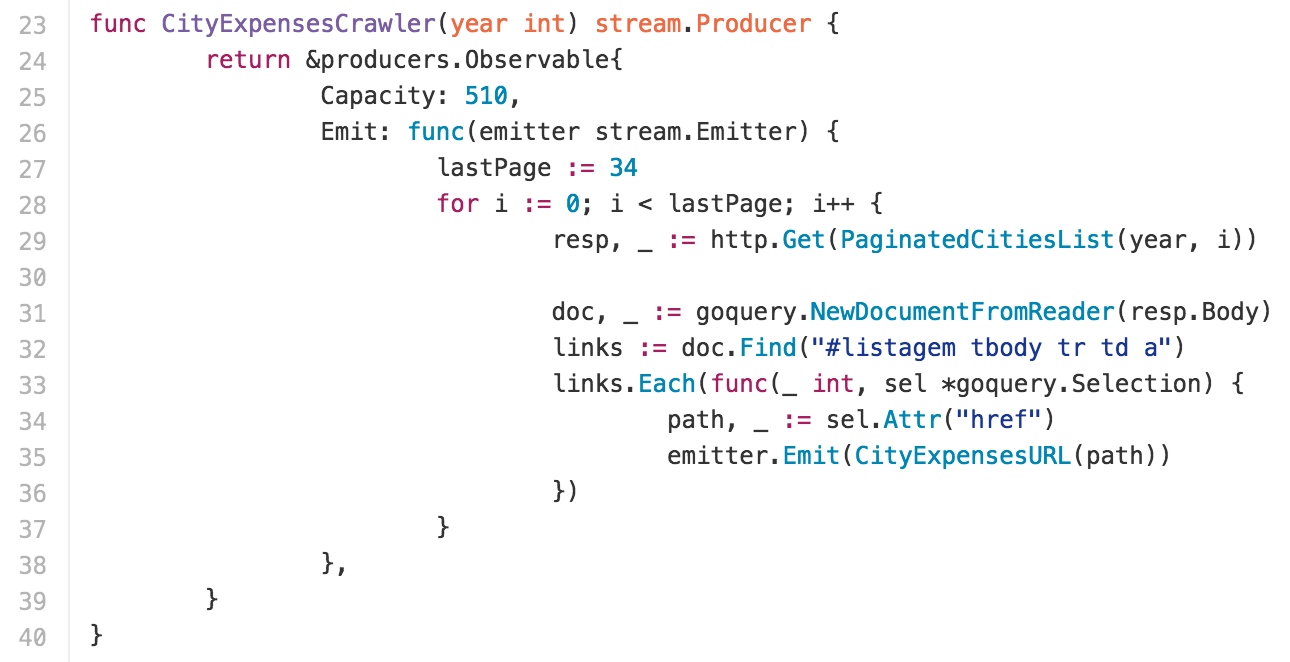
\includegraphics[width=1\textwidth]{crawler}
  \centering
  \caption{Exemplo de um Crawler que implementa a interface stream.Producer.}
  \label{code:crawler}
\end{figure}

\begin{figure}[H]
  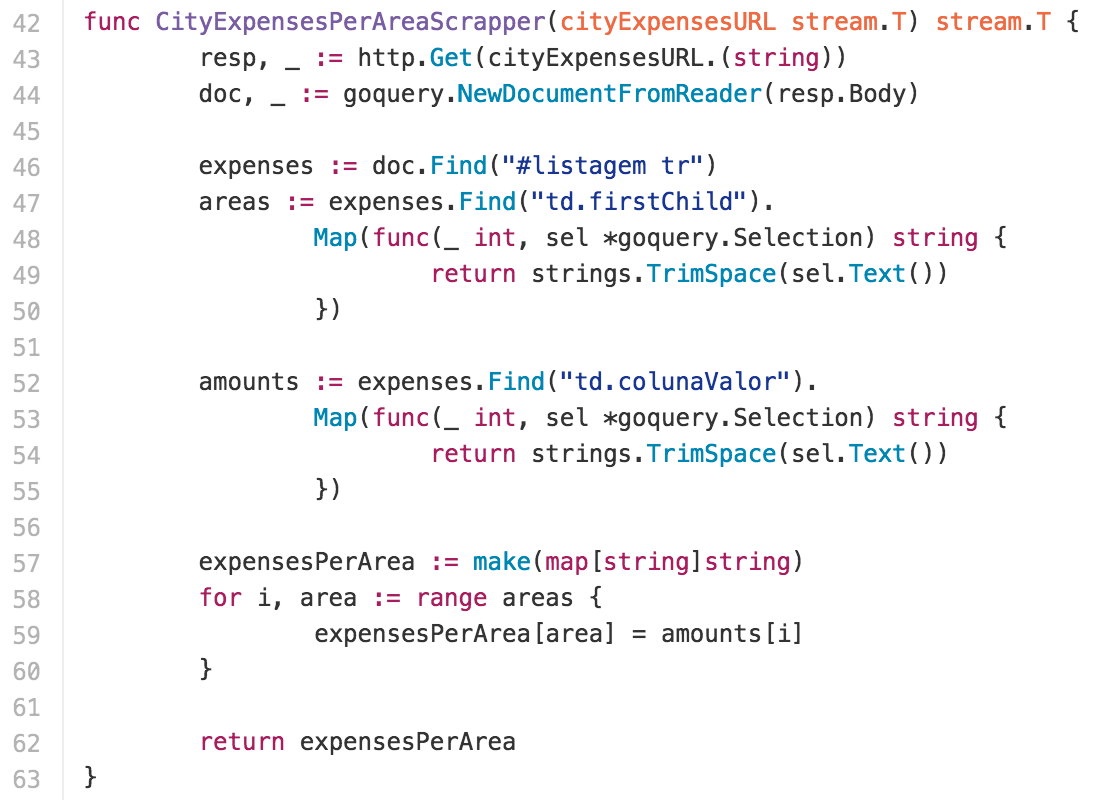
\includegraphics[width=1\textwidth]{scrapper}
  \centering
  \caption{Exemplo de um Scrapper que implementa a interface stream.Transformer.}
  \label{code:scrapper}
\end{figure}

\begin{figure}[H]
  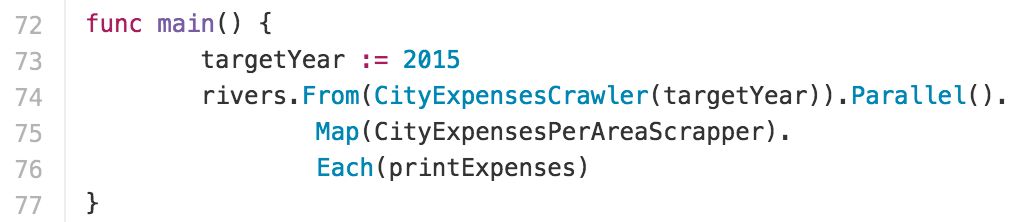
\includegraphics[width=1\textwidth]{scrapping_example}
  \centering
  \caption{Exemplo de uso do Crawler e Scrapper em um pipeline Rivers.}
  \label{code:scrapping_example}
\end{figure}

\chapter{Conclusão}
\label{cha:conclusion}

Rivers propões uma API simples, extensível e intuitiva para processamento de streams de dados para a linguagem Go, utilizando de construções e conceitos de programação funcional familiares a maioria dos desenvolvedores abstraindo as complexidades e detalhes de implementação relacionados ao processamento concorrente e paralelo dos dados, de maneira que o desenvolvedor passa se concentrar apenas na lógica de negócio intrínseca ao pipeline.

O modelo de concorrência da linguagem Go provou-se não somente muito conveniente mas também extremamente eficiente e foi crucial para o sucesso da implementação da solução uma vez que muito da complexidade dos mecanismos de detecção de falhas, de comunicação entre os componentes do sistema via channels e gerência de recursos alocados durante a execução de grandes quantidades de fluxos de processamento concorrentes não afetaram de maneira considerável a complexidade final da solução.

Por se tratar de um experimento e guiado inicialmente pelas necessidades e casos de uso da emprese Bearch Inc, a API sofreu várias alterações ao longo do desenvolvimento afim de adaptá-la a novos casos de uso, porém visando simplicidade algumas operações encontradas em APIs similares em outras plataformas não foram implementadas como por exemplo determinados tipos de operações de filtros que no entanto podem ser implementadas através da composição de outras operações disponíveis na API.

\section{Análise dos Resultados}
\label{sec:results}

Ao longo do desenvolvimento muitas informações foram coletadas desde benchmarks até feedbacks de desenvolvedores utilizando o framework em outros projetos da empresa afim de avaliar a solução em termos de performance, simplicidade e flexibilidade. Os resultados dos benchmarks foram muito satisfatórios e mostraram um ganho considerável em performance ao se paralelizar estágios do pipeline além da execução concorrente de cada estágio.

O design funcional da API agradou desenvolvedores pela simplicidade da solução e o fato de se poder estender a API com novos componentes implementando as interfaces definidas pelo framework possibilitou o uso de Rivers em contextos bem variados. Algumas das decisões técnicas quanto ao design da API foram guiados por feedbacks de usuários que alongo de várias conversas e experimentos ajudaram a moldar a API final desde a nomenclatura das operações até mesmo com relação a melhor solução para se paralelizar pipelines sem expor qualquer tipo de complexidade ao usuário do framework. Um ponto negativo levantado por desenvolvedores é que devido ao fato da sintaxe da linguagem Go em alguns aspectos é um pouco extensa comparado com outras soluções em outras linguagens como scala e python, é necessário escrever um pouco mais de código, porém isso pode ser contornado fornecendo implementações específicas de operações recorrentes que possam ser reusadas evitando a necessidade de se implementar a mesma funcionalidade em diferentes contextos.

\section{Trabalhos Futuros}
\label{sec:future_work}

Ao longo do desenvolvimento da solução, alguns casos de uso interessantes foram detectados, propostos e discutidos como por exemplo a possibilidade de se implementar pipelines distribuídos, permitindo a execução de diferentes estágios do pipeline em um cluster de máquinas seguindo um modelo similar ao modelo MapReduce proposto por Google \cite{paper:google:map_reduce}. Apesar de ser um caso de uso muito interessante, a complexidade de implementação não justificou sua necessidade momentânea e portanto não foi considerado prioridade no desenvolvimento. Porém essa possibilidade não foi completamente descartada e fica proposta como trabalho futuro uma vez que existem necessidades reais que justificam o investimento em tal solução, especialmente nos domínios de Big Data aonde o volume de dados a serem processados é incrivelmente grande e a possibilidade de se distribuir e processar conjuntos menores destes dados em diferentes máquinas agregando seus resultados ao final é muito atraente.

%
% ---------------------------------------------------------
%

\bibliographystyle{abntex2-alf}
\bibliography{biblio}

\end{document}
